% Options for packages loaded elsewhere
\PassOptionsToPackage{unicode}{hyperref}
\PassOptionsToPackage{hyphens}{url}
%
\documentclass[
]{article}
\usepackage{amsmath,amssymb}
\usepackage{lmodern}
\usepackage{iftex}
\ifPDFTeX
  \usepackage[T1]{fontenc}
  \usepackage[utf8]{inputenc}
  \usepackage{textcomp} % provide euro and other symbols
\else % if luatex or xetex
  \usepackage{unicode-math}
  \defaultfontfeatures{Scale=MatchLowercase}
  \defaultfontfeatures[\rmfamily]{Ligatures=TeX,Scale=1}
\fi
% Use upquote if available, for straight quotes in verbatim environments
\IfFileExists{upquote.sty}{\usepackage{upquote}}{}
\IfFileExists{microtype.sty}{% use microtype if available
  \usepackage[]{microtype}
  \UseMicrotypeSet[protrusion]{basicmath} % disable protrusion for tt fonts
}{}
\makeatletter
\@ifundefined{KOMAClassName}{% if non-KOMA class
  \IfFileExists{parskip.sty}{%
    \usepackage{parskip}
  }{% else
    \setlength{\parindent}{0pt}
    \setlength{\parskip}{6pt plus 2pt minus 1pt}}
}{% if KOMA class
  \KOMAoptions{parskip=half}}
\makeatother
\usepackage{xcolor}
\IfFileExists{xurl.sty}{\usepackage{xurl}}{} % add URL line breaks if available
\IfFileExists{bookmark.sty}{\usepackage{bookmark}}{\usepackage{hyperref}}
\hypersetup{
  pdfauthor={Timothy J. Miller1,2; Kiersten L. Curti1,3; Alexander C. Hansell1,4},
  hidelinks,
  pdfcreator={LaTeX via pandoc}}
\urlstyle{same} % disable monospaced font for URLs
\usepackage[margin=1in]{geometry}
\usepackage{longtable,booktabs,array}
\usepackage{calc} % for calculating minipage widths
% Correct order of tables after \paragraph or \subparagraph
\usepackage{etoolbox}
\makeatletter
\patchcmd\longtable{\par}{\if@noskipsec\mbox{}\fi\par}{}{}
\makeatother
% Allow footnotes in longtable head/foot
\IfFileExists{footnotehyper.sty}{\usepackage{footnotehyper}}{\usepackage{footnote}}
\makesavenoteenv{longtable}
\usepackage{graphicx}
\makeatletter
\def\maxwidth{\ifdim\Gin@nat@width>\linewidth\linewidth\else\Gin@nat@width\fi}
\def\maxheight{\ifdim\Gin@nat@height>\textheight\textheight\else\Gin@nat@height\fi}
\makeatother
% Scale images if necessary, so that they will not overflow the page
% margins by default, and it is still possible to overwrite the defaults
% using explicit options in \includegraphics[width, height, ...]{}
\setkeys{Gin}{width=\maxwidth,height=\maxheight,keepaspectratio}
% Set default figure placement to htbp
\makeatletter
\def\fps@figure{htbp}
\makeatother
\setlength{\emergencystretch}{3em} % prevent overfull lines
\providecommand{\tightlist}{%
  \setlength{\itemsep}{0pt}\setlength{\parskip}{0pt}}
\setcounter{secnumdepth}{5}
\newlength{\cslhangindent}
\setlength{\cslhangindent}{1.5em}
\newlength{\csllabelwidth}
\setlength{\csllabelwidth}{3em}
\newlength{\cslentryspacingunit} % times entry-spacing
\setlength{\cslentryspacingunit}{\parskip}
\newenvironment{CSLReferences}[2] % #1 hanging-ident, #2 entry spacing
 {% don't indent paragraphs
  \setlength{\parindent}{0pt}
  % turn on hanging indent if param 1 is 1
  \ifodd #1
  \let\oldpar\par
  \def\par{\hangindent=\cslhangindent\oldpar}
  \fi
  % set entry spacing
  \setlength{\parskip}{#2\cslentryspacingunit}
 }%
 {}
\usepackage{calc}
\newcommand{\CSLBlock}[1]{#1\hfill\break}
\newcommand{\CSLLeftMargin}[1]{\parbox[t]{\csllabelwidth}{#1}}
\newcommand{\CSLRightInline}[1]{\parbox[t]{\linewidth - \csllabelwidth}{#1}\break}
\newcommand{\CSLIndent}[1]{\hspace{\cslhangindent}#1}
\usepackage{url}
\usepackage{setspace}
%\singlespacing
%\onehalfspacing
%\doublespacing
\usepackage{lineno}
%\linenumbers
\usepackage[belowskip=0pt,aboveskip=0pt]{caption}
\usepackage{relsize}
\usepackage{float}
% \usepackage[section]{placeins}
\usepackage{lscape}
\usepackage{longtable}
\usepackage{amsmath,rotating}
\usepackage[scanall]{psfrag}
\usepackage{bm}
\usepackage{caption,graphics}
\usepackage{graphicx}
%\usepackage{natbib}
%\usepackage[nottoc]{tocbibind}
%\usepackage{indentfirst}
\usepackage{sectsty}
\usepackage{color}
\usepackage{fancyhdr}
\usepackage{xspace}
\usepackage{textcomp}
\usepackage{upgreek}
% \usepackage{xr}
% \externaldocument{supp_final}
\newcommand{\blandscape}{\begin{landscape}}
\newcommand{\elandscape}{\end{landscape}}
\newcommand{\noop}[1]{}
\usepackage{booktabs}
\usepackage{longtable}
\usepackage{array}
\usepackage{multirow}
\usepackage{wrapfig}
\usepackage{float}
\usepackage{colortbl}
\usepackage{pdflscape}
\usepackage{tabu}
\usepackage{threeparttable}
\usepackage{threeparttablex}
\usepackage[normalem]{ulem}
\usepackage{makecell}
\usepackage{xcolor}
\ifLuaTeX
  \usepackage{selnolig}  % disable illegal ligatures
\fi

\title{~Space for WHAM: a multi-region, multi-stock generalization of the Woods Hole Assessment Model with an application to black sea bass:\\
\hspace*{0.333em}Supplementary Materials}
\author{Timothy J. Miller\textsuperscript{1,2} \and Kiersten L. Curti\textsuperscript{1,3} \and Alexander C. Hansell\textsuperscript{1,4}}
\date{}

\begin{document}
\maketitle

\(1\) Northeast Fisheries Science Center, National Marine Fisheries Service, 166 Water Street, Woods Hole, MA 02543, USA\\
\(2\) orcid: 0000-0003-1411-1206, \href{mailto:timothy.j.miller@noaa.gov}{\nolinkurl{timothy.j.miller@noaa.gov}}\\
\(3\) orcid: 0009-0009-1676-7269\\
\(4\) orcid: 0000-0001-7827-1749\\

\pagebreak

\hypertarget{deriving-the-prior-distribution-for-movement-parameters}{%
\subsection*{Deriving the prior distribution for movement parameters}\label{deriving-the-prior-distribution-for-movement-parameters}}
\addcontentsline{toc}{subsection}{Deriving the prior distribution for movement parameters}

The Working Group fit a Stock Synthesis model (\protect\hyperlink{ref-methotwetzel13}{Methot and Wetzel 2013}) that included tagging data with 2 seasons (6 months each) and 2 regions where a proportion \(\mu^*_1\) of the northern component moves to the south in one season and some proportion \(\mu^*_{2\rightarrow 1}\) move back to the south in the second season (\protect\hyperlink{ref-nefsc23}{NEFSC 2023}). The seasonal movement matrices for each season are
\begin{equation*}
\boldsymbol{\mu}^*_{1} = 
  \begin{bmatrix}
     1-\mu^*_{1\rightarrow 2} & \mu^*_{1\rightarrow 2} \\
     0 & 1 \\
  \end{bmatrix}
\end{equation*}
and
\begin{equation*}
\boldsymbol{\mu}_{2} = 
  \begin{bmatrix}
     1 &  0 \\
     \mu^*_{2\rightarrow 1} & 1-\mu^*_{2\rightarrow 1} \\
  \end{bmatrix}.
\end{equation*}

To obtain estimates of movement proportions for the monthly intervals in the WHAM model, the half-year movement matrices were converted to monthly movement matrices by taking the root \(z_k\) of \(\boldsymbol{\mu}^*_{k}\) which are defined by the number of months of movement for each season (5 and 4, respectively). The roots of the matrices are calculated using an eigen decomposition of the matrices
\[ \boldsymbol{\mu}_k =  \left(\boldsymbol{\mu}_k^*\right)^{z_k} = \mathbf{V}_k \mathbf{D}_k^{z_k} \mathbf{V}_k^{-1},\]
where \(z_1 = 1/5\) for and \(z_2 = 1/4\), and \(\mathbf{V}_{k}\) and \(\mathbf{D}_{k}\) are the matrix of eigenvectors (columnwise) and the diagonal matrix of corresponding eigenvalues of \(\boldsymbol{\mu}^*_k\). The Working Group used a parametric bootstrap approach to determine an appropriate standard deviation for the prior distribution for the movement parameters. Stock Synthesis also estimates parameters on a transformed scale, but different from WHAM:
\[\mu^*_{r\rightarrow r'} = \frac{1}{1 + 2e^{-x_{r\rightarrow r'}}}\]
The estimated parameters and standard errors from the Stock Synthesis model were \(x_{1\rightarrow 2}=-1.44\) and \(x_{2\rightarrow 1}=1.94\) and \(SE(x_{1\rightarrow 2})) = 0.21\) and \(SE(x_{2\rightarrow 1})) = 0.37\). The resulting in the estimated proportions were \(\mu^*_{1\rightarrow 2}=0.11\) and \(\mu^*_{2\rightarrow 1}=0.78\).

In WHAM, an additive logit transformation is used which is simply a logit transformation when there are only two regions:
\[
\mu_{r\rightarrow r'} = \frac{1}{1+e^{-y_{r\rightarrow r'}}}.
\]
We simulated 1000 values from a normal distribution with mean and standard deviation defined by the parameter estimate and standard error \(\tilde x_{{r\rightarrow r'},b} \sim N(x_{r\rightarrow r'}, SE(x_{r\rightarrow r'}))\) from the Stock Synthesis model. For each simulated value we constructed \(\tilde {\boldsymbol{\mu}}^*_{{r\rightarrow r'},b}\), took the appropriate root and calculated inverse logit for \(\tilde y_{{r\rightarrow r'},b}\). We calculated the mean and standard deviation of the values \(y_{i,b}\). The mean values did not differ meaningfully from the transformation of the original estimates (\(y_{1\rightarrow 2} = -3.79\) and \(y_{2\rightarrow 1} = -0.79\)) and the standard deviation was approximately 0.2 for both parameters.

\hypertarget{bottom-temperature-anomalies}{%
\subsection*{Bottom temperature anomalies}\label{bottom-temperature-anomalies}}
\addcontentsline{toc}{subsection}{Bottom temperature anomalies}

The Working Group created bottom temperature observations from a high resolution ocean bottom temperature product by du Pontavice et al. (\protect\hyperlink{ref-dupontaviceetal23}{2023}). The annual observations for each region are defined by the average over all spatial bottom temperature values for February and March by region and year. Similarly, the Working Group calculated standard errors from the standard deviation of all values in the region and the total number of values for a given year. We created regional bottom temperature anomalies by subtracting means for each region across all years.

\hypertarget{diagnostics}{%
\subsection*{Diagnostics}\label{diagnostics}}
\addcontentsline{toc}{subsection}{Diagnostics}

\hypertarget{jitter-fits-for-model-m_0}{%
\subsubsection*{\texorpdfstring{Jitter fits for model \(M_0\)}{Jitter fits for model M\_0}}\label{jitter-fits-for-model-m_0}}
\addcontentsline{toc}{subsubsection}{Jitter fits for model \(M_0\)}

WHAM by default completes three newton steps after the stats::nlminb minimization function completes to reduce the gradient at the minimized NLL. However, this generally has negligible effects on model estimates and the NLL. To reduce computation time, we did not complete these newton steps when performing jitter fits of the model. Without the Newton steps, the maximum (absolute) gradient sizes are generally less than 0.01 for models that converge satisfactorily.

The 50 jitter fits demonstrated that a local minimum was obtained for the original fit of model \(M_0\) (Figure \ref{fig:jitter-M0}). One lower NLL was obtained with unacceptable gradients (No.~25), but a slightly lower NLL was found with a satisfactory gradient for 3 of the jitters (Nos. 9, 13, 29). However, one of the jitter fits (No.~9) did not provide a non-zero estimate of the variance parameter for one of the indices and the other two provided identical results and we refit model \(M_0\) and all remaining models using the better parameter estimates as initial values.

\hypertarget{jitter-fits-for-model-m_1}{%
\subsubsection*{\texorpdfstring{Jitter fits for model \(M_1\)}{Jitter fits for model M\_1}}\label{jitter-fits-for-model-m_1}}
\addcontentsline{toc}{subsubsection}{Jitter fits for model \(M_1\)}

The 50 jitter fits gave no evidence of a better minimization of the NLL. Three lower NLLs were obtained, but with unacceptably large gradients (Figure \ref{fig:jitter-M1}). The largest differences in parameter estimates for these three jitters were for numbers at age and selectivity random effects variance and correlation parameters.

\hypertarget{self-test-for-model-m_1}{%
\subsubsection*{\texorpdfstring{Self test for model \(M_1\)}{Self test for model M\_1}}\label{self-test-for-model-m_1}}
\addcontentsline{toc}{subsubsection}{Self test for model \(M_1\)}

Initial fits to simulated data from model \(M_1\) showed estimation of the observation error standard deviation multiplier for the recreational catch-per angler indices in the north and south regions was unstable. Many of the fits to the simulated data produced implausible estimates at the 0 boundary for these parameters (very negative values on log-scale). However, across all fits including those with poor convergence, estimation of SSB and fishing mortality was reliable (Figure \ref{fig:self-test-fig}). We also fit analogous models with the multiplier parameters fixed at the true values, which did improve convergence, but larger bias was estimated for fishing mortality and SSB for the northern component.

\hypertarget{references}{%
\section*{References}\label{references}}
\addcontentsline{toc}{section}{References}

\hypertarget{refs}{}
\begin{CSLReferences}{1}{0}
\leavevmode\vadjust pre{\hypertarget{ref-dupontaviceetal23}{}}%
du Pontavice, H., Chen, Z., and Saba, V.S. 2023. A high-resolution ocean bottom temperature product for the northeast {U}.{S}. Continental shelf marine ecosystem. Progress in Oceanography \textbf{210}: 102948. doi:\href{https://doi.org/10.1016/j.pocean.2022.102948}{10.1016/j.pocean.2022.102948}.

\leavevmode\vadjust pre{\hypertarget{ref-methotwetzel13}{}}%
Methot, R.D., and Wetzel, C.R. 2013. Stock {S}ynthesis: A biological and statistical framework for fish stock assessment and fishery management. Fisheries Research \textbf{142}(1): 86--99. doi:\href{https://doi.org/10.1016/j.fishres.2012.10.012}{10.1016/j.fishres.2012.10.012}.

\leavevmode\vadjust pre{\hypertarget{ref-nefsc23}{}}%
NEFSC. 2023. Report of the black sea bass (\emph{{C}entropristis} \emph{striata}) research track stock assessment working group. {Available} at https://www.mafmc.org/s/a\_2023\_BSB\_UNIT\_RTWG\_Report\_V2\_12\_2\_2023-1.pdf.

\end{CSLReferences}

\pagebreak

\setcounter{table}{0}
\renewcommand\thetable{S\arabic{table}}

\begin{landscape}\begin{table}

\caption{\label{tab:age-comp-sel-table}Configuration of age composition likelihoods, mean selectivity models, and selectivity random effects models for each age composition data component. For all logistic-normal likelihoods, any ages observed as zeros are treated as missing.}
\centering
\begin{tabular}[t]{llll}
\toprule
Data component & Age Composition Likelihood & Mean Selectivity model & Random effects Model\\
\midrule
North commercial fleet & Dirichlet-Multinomial & age-specific (ages > 3 fully selected) & AR1 correlation by age and year\\
North recreational fleet & Logistic-normal (Independent) & age-specific (ages > 6 fully selected) & AR1 correlation by age and year\\
South commercial fleet & Logistic-normal (AR1 correlation) & logistic & None\\
South recreational fleet & Logistic-normal (AR1 correlation) & logistic & None\\
North recreational CPA index & Logistic-normal (Independent) & age-specific (ages > 1 fully selected) & AR1 correlation by year\\
\addlinespace
North VAST index & Dirichlet-Multinomial & age-specific (ages > 4 fully selected) & AR1 correlation by age and year\\
South recreational CPA index & Logistic-normal (AR1 correlation) & age-specific (ages > 2 fully selected) & None\\
South VAST index & Logistic-normal (AR1 correlation) & age-specific (ages > 1 fully selected) & None\\
\bottomrule
\end{tabular}
\end{table}
\end{landscape}

\begin{table}

\caption{\label{tab:aic-wts-table}Model AIC weights for each retrospective peel.}
\centering
\begin{tabular}[t]{lrrrrrrrr}
\toprule
\multicolumn{1}{c}{ } & \multicolumn{8}{c}{Peel} \\
\cmidrule(l{3pt}r{3pt}){2-9}
Model & 0 & 1 & 2 & 3 & 4 & 5 & 6 & 7\\
\midrule
$M_{0}$ & 0.00 & 0.00 & 0.00 & 0.00 & 0.00 & 0.00 & 0.01 & 0.01\\
$M_{1}$ & 0.45 & 0.43 & 0.42 & 0.38 & 0.41 & 0.37 & 0.36 & 0.38\\
$M_{2}$ & 0.00 & 0.00 & 0.00 & 0.00 & 0.00 & 0.00 & 0.00 & 0.00\\
$M_{3}$ & 0.30 & 0.31 & 0.25 & 0.23 & 0.24 & 0.23 & 0.25 & 0.23\\
$M_{4}$ & 0.00 & 0.00 & 0.00 & 0.00 & 0.00 & 0.00 & 0.00 & 0.00\\
\addlinespace
$M_{5}$ & 0.00 & 0.00 & 0.00 & 0.00 & 0.00 & 0.00 & 0.00 & 0.00\\
$M_{6}$ & 0.00 & 0.00 & 0.00 & 0.00 & 0.00 & 0.00 & 0.00 & 0.00\\
$M_{7}$ & 0.00 & 0.00 & 0.00 & 0.00 & 0.00 & 0.00 & 0.00 & 0.00\\
$M_{8}$ & 0.15 & 0.15 & 0.20 & 0.24 & 0.21 & 0.24 & 0.22 & 0.23\\
$M_{9}$ & 0.00 & 0.00 & 0.00 & 0.00 & 0.00 & 0.00 & 0.00 & 0.00\\
\addlinespace
$M_{10}$ & 0.10 & 0.11 & 0.12 & 0.14 & 0.13 & 0.15 & 0.15 & 0.14\\
$M_{11}$ & 0.00 & 0.00 & 0.00 & 0.00 & 0.00 & 0.00 & 0.00 & 0.00\\
$M_{12}$ & 0.00 & 0.00 & 0.00 & 0.00 & 0.00 & 0.00 & 0.00 & 0.00\\
$M_{13}$ & 0.00 & 0.00 & 0.00 & 0.00 & 0.00 & 0.00 & 0.00 & 0.00\\
\bottomrule
\end{tabular}
\end{table}

\setcounter{figure}{0}
\renewcommand\thefigure{S\arabic{figure}}

\pagebreak

\begin{figure}

{\centering 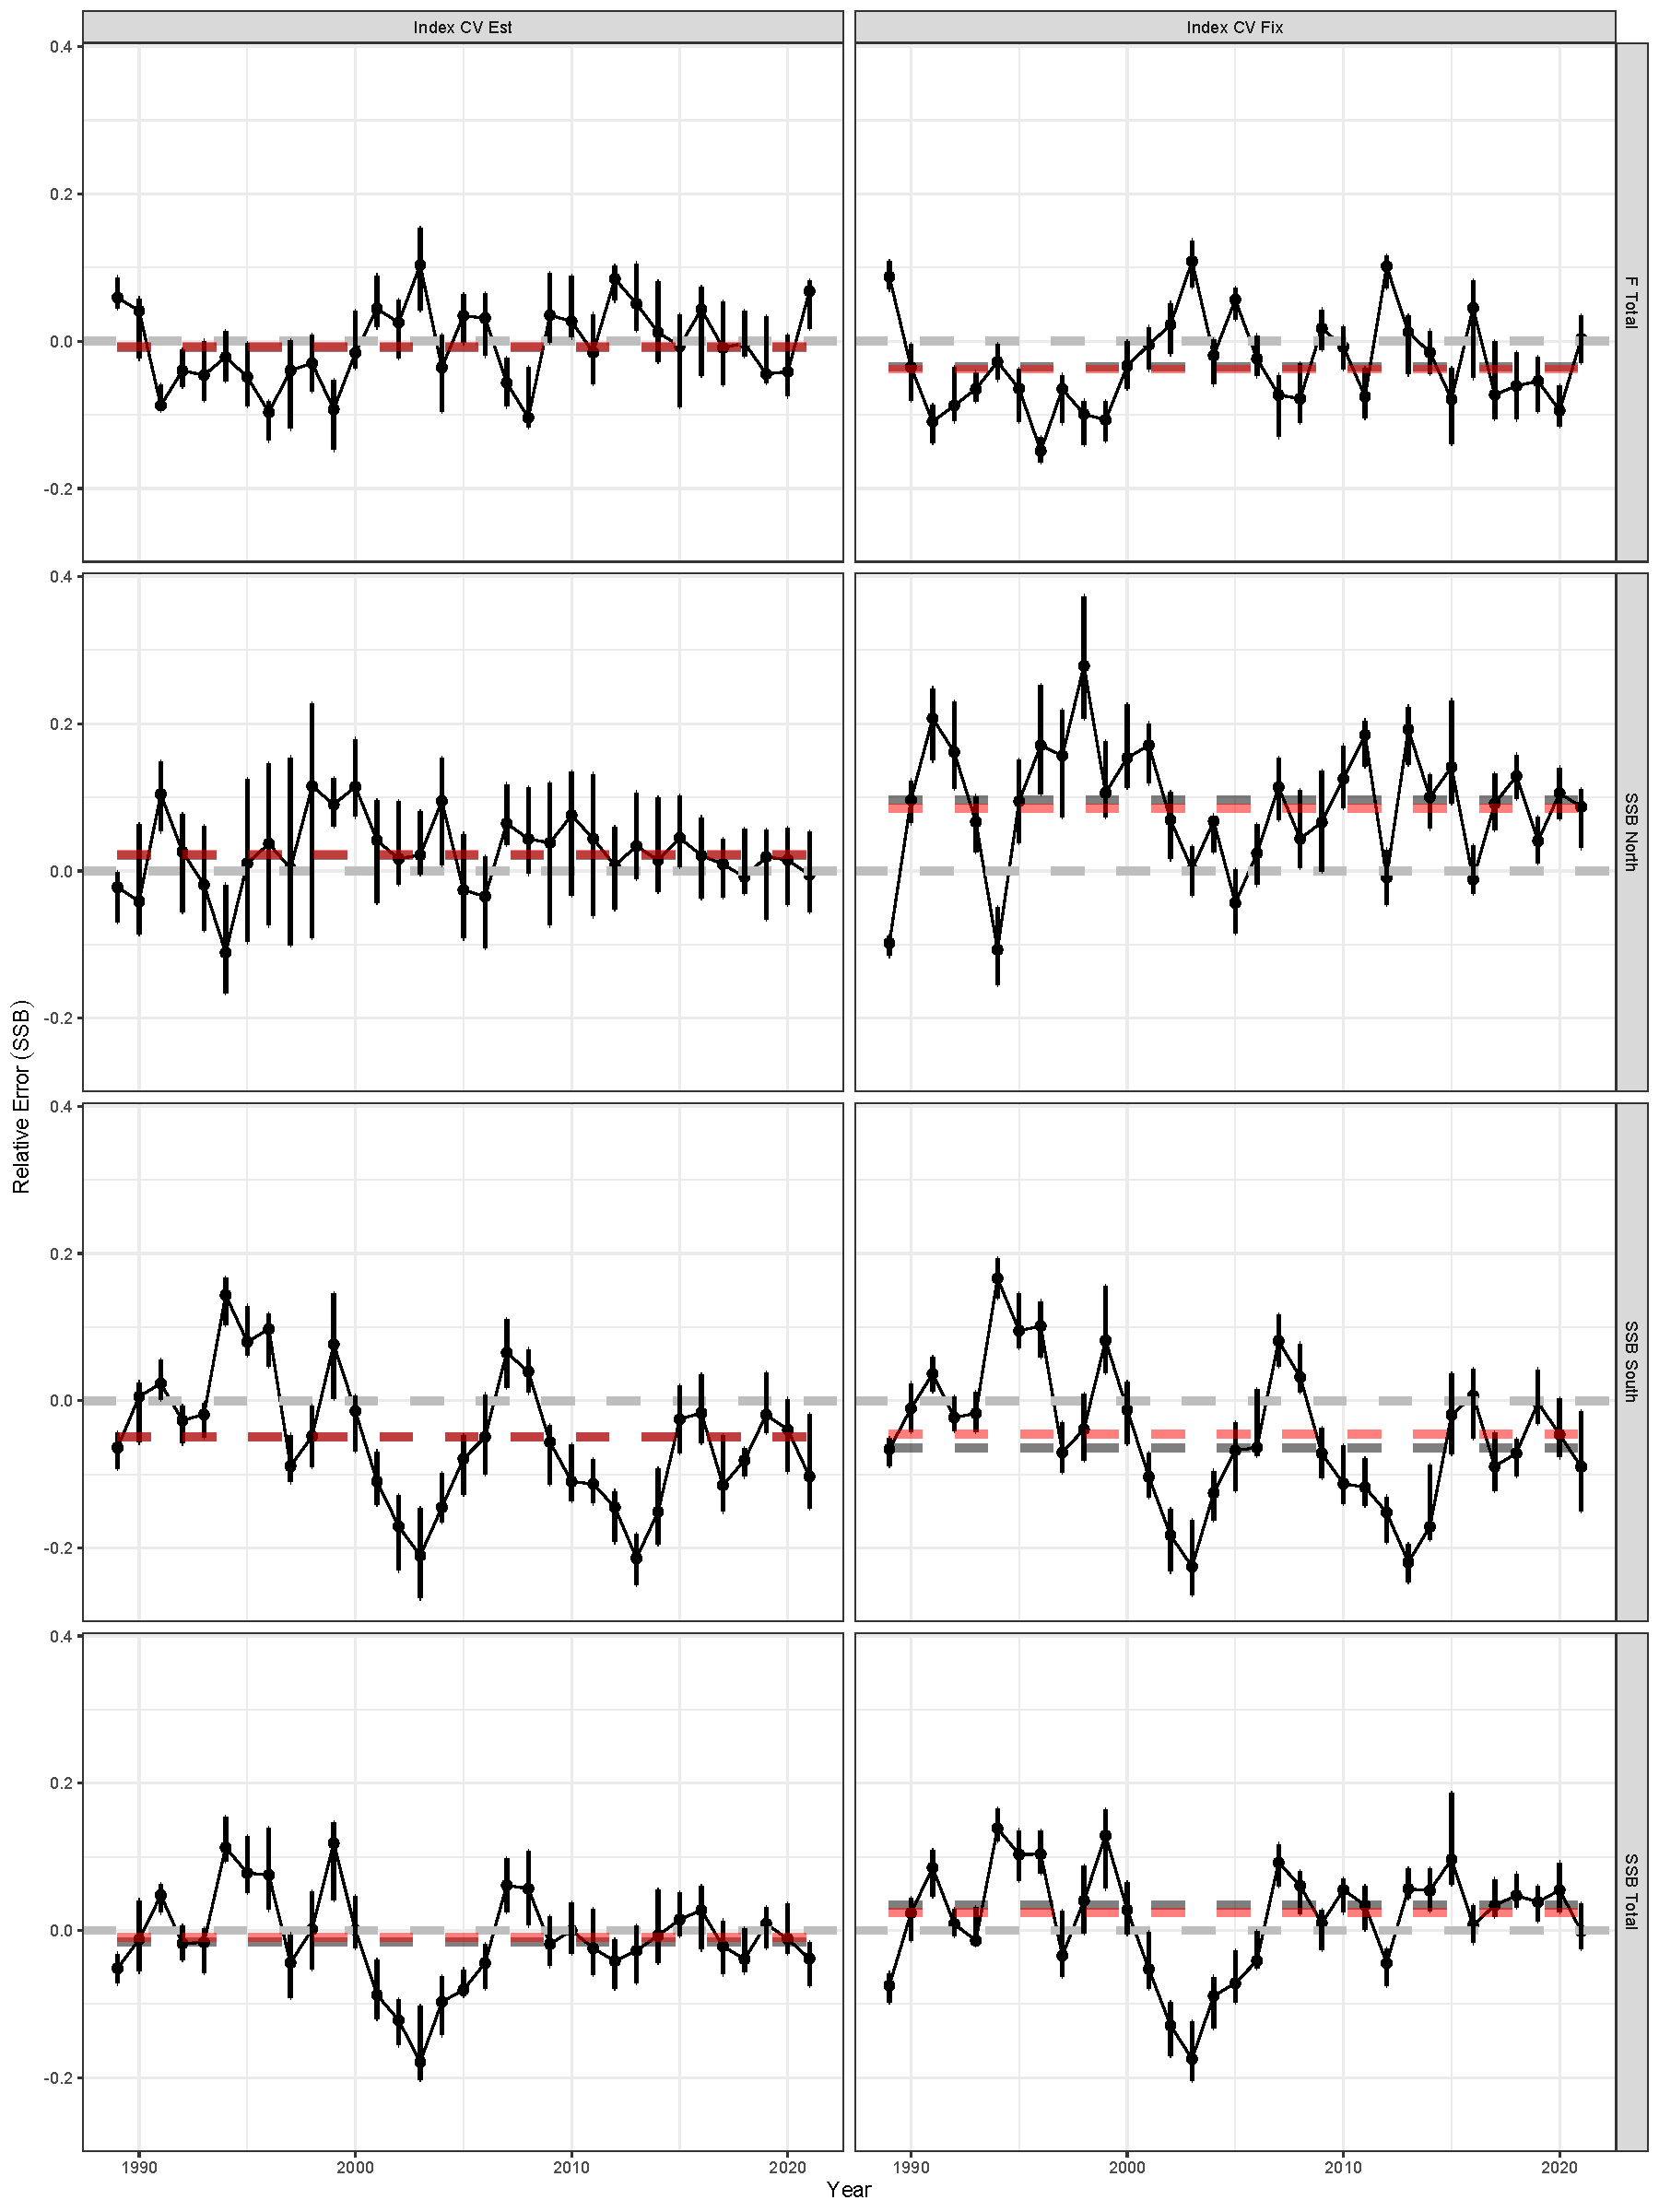
\includegraphics[width=1\linewidth]{self_test_results} 

}

\caption{Median relative error of SSB (Total and by stock component) and total fully-selected fishing mortality for estimation models fitted to simulated data from model $M_1$ where the observation variance of log-indices are fixed and estimated. Black and Red dashed lines represent the median of the annual medians and the median across all annual relative errors, respectively. Vertical lines represent 95\% confidence intervals.}\label{fig:self-test-fig}
\end{figure}

\begin{figure}

{\centering 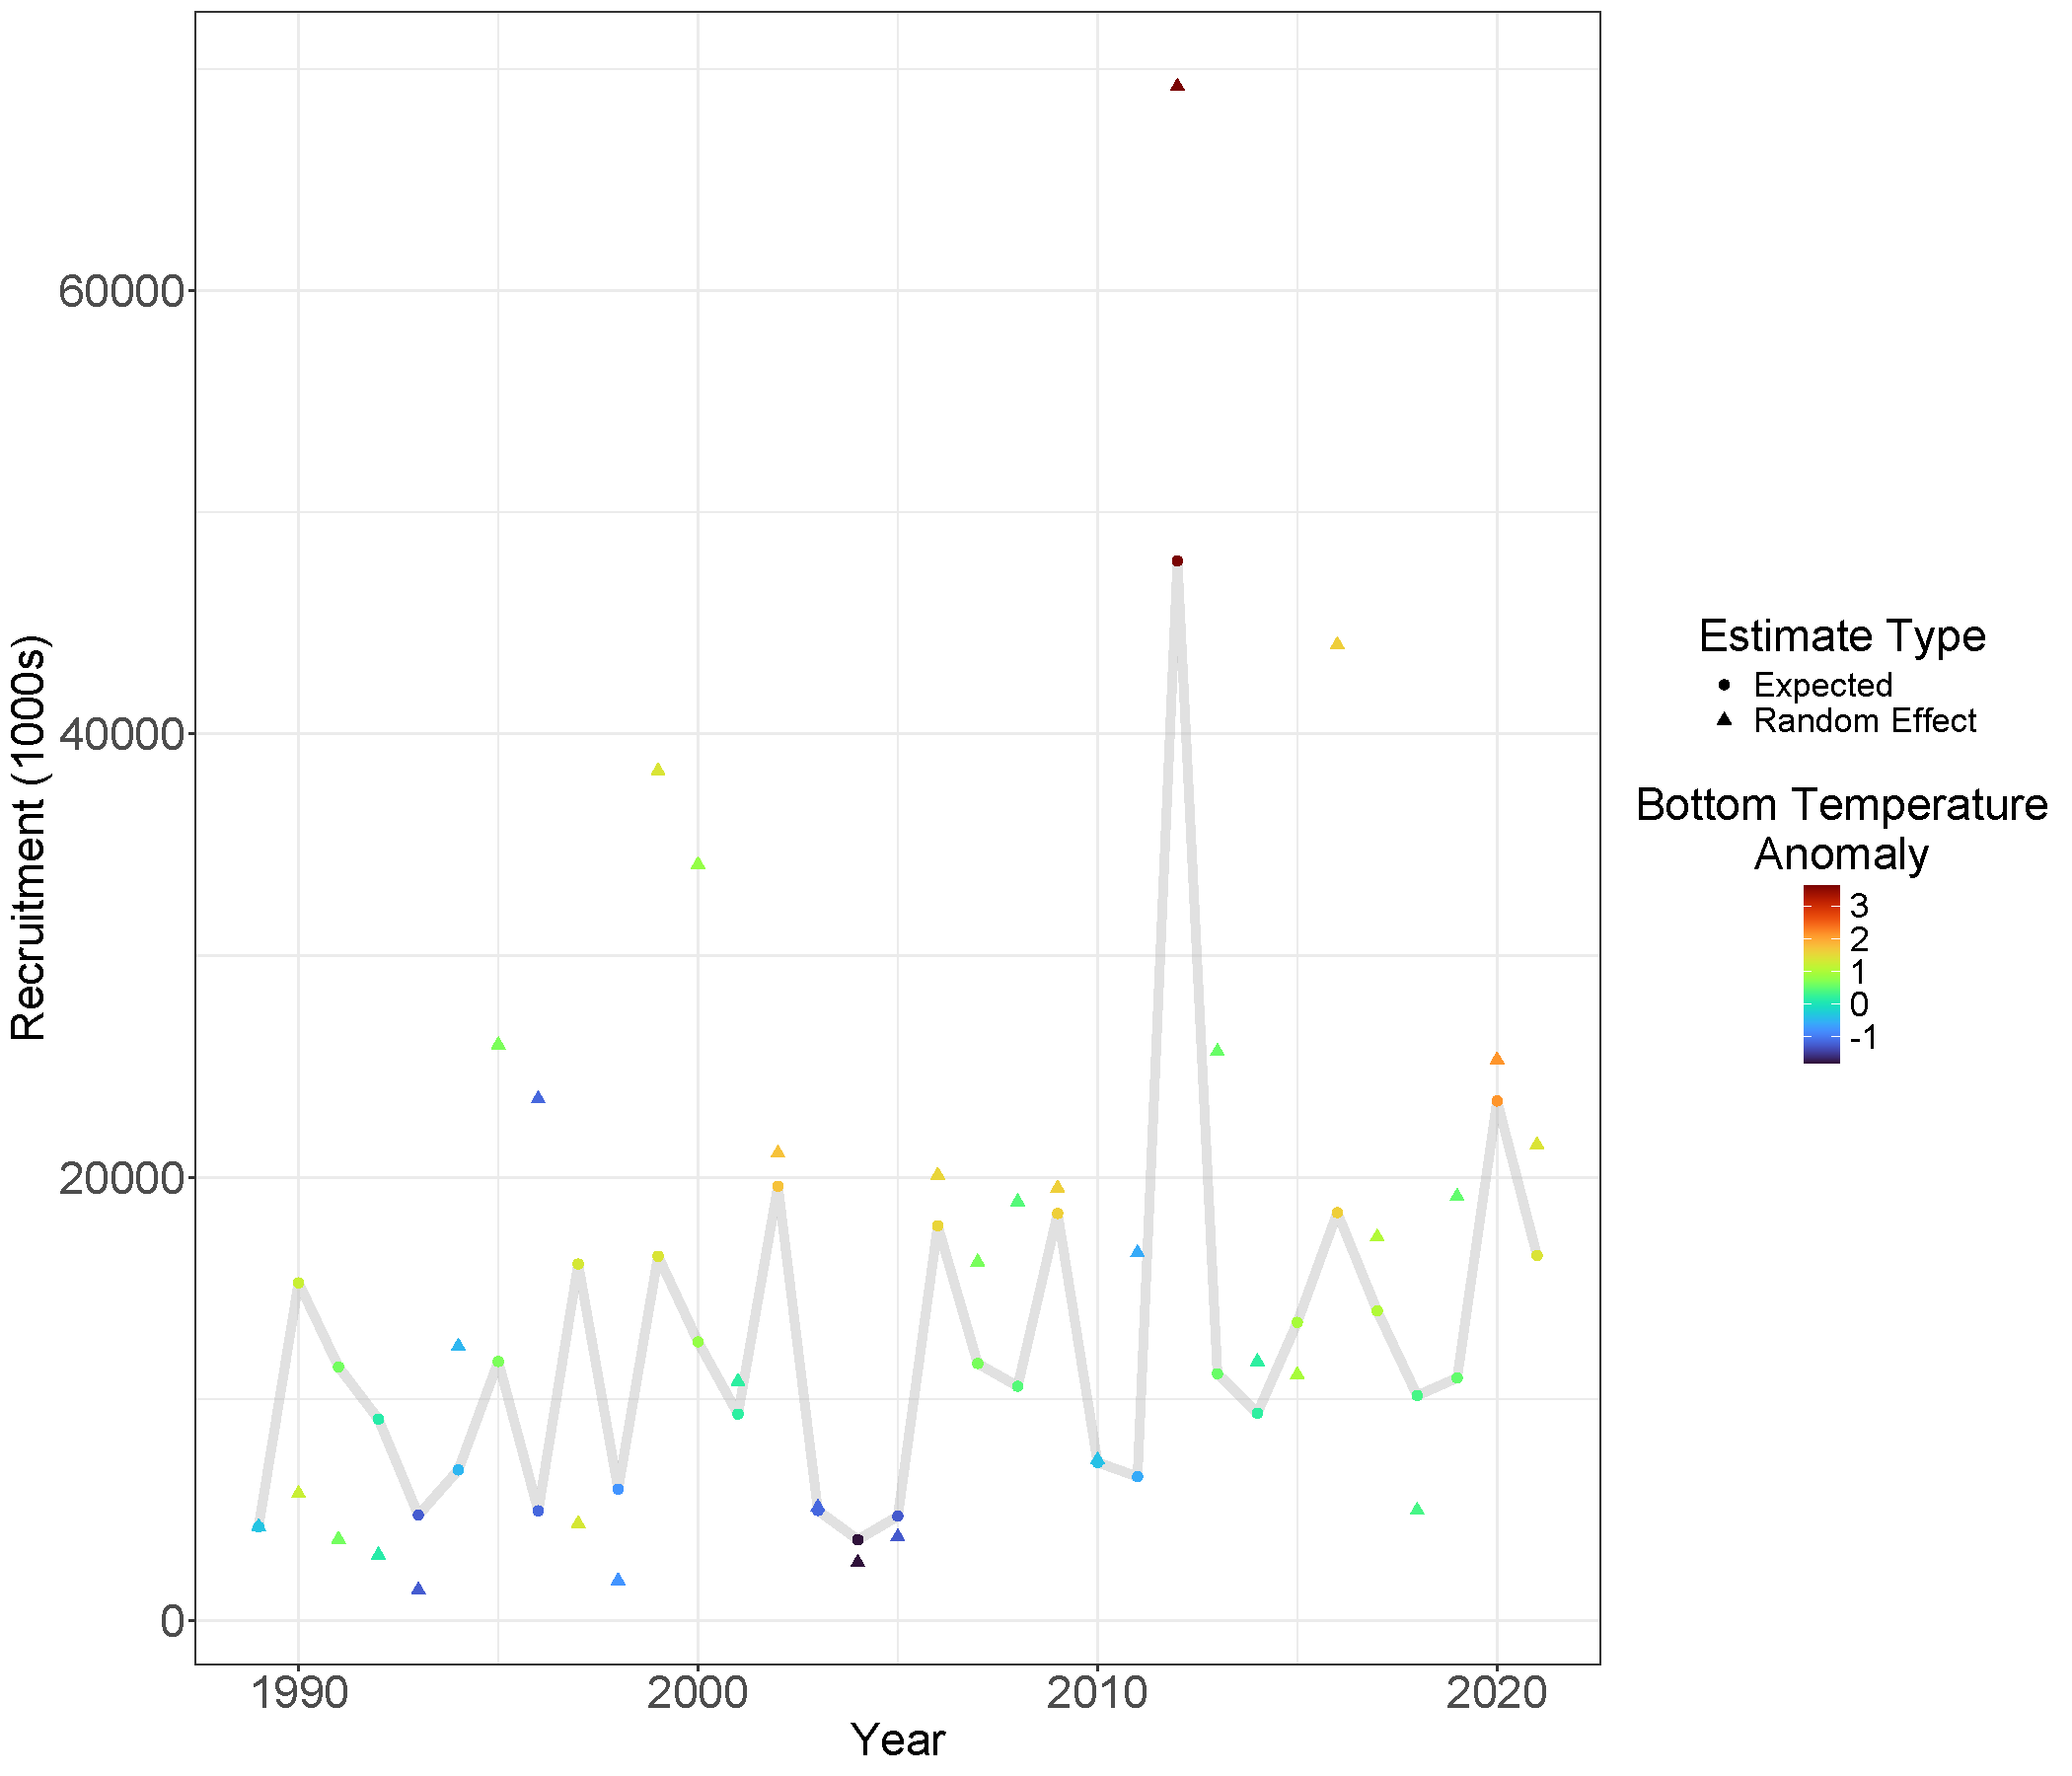
\includegraphics[width=1\linewidth]{best_R_Ecov} 

}

\caption{Expected and random effect recruitment estimates for the northern stock component. Color of points defined by the corresponding annual bottom temperature anomaly.}\label{fig:BT-Ecov-R}
\end{figure}

\begin{landscape}
\begin{figure}

{\centering 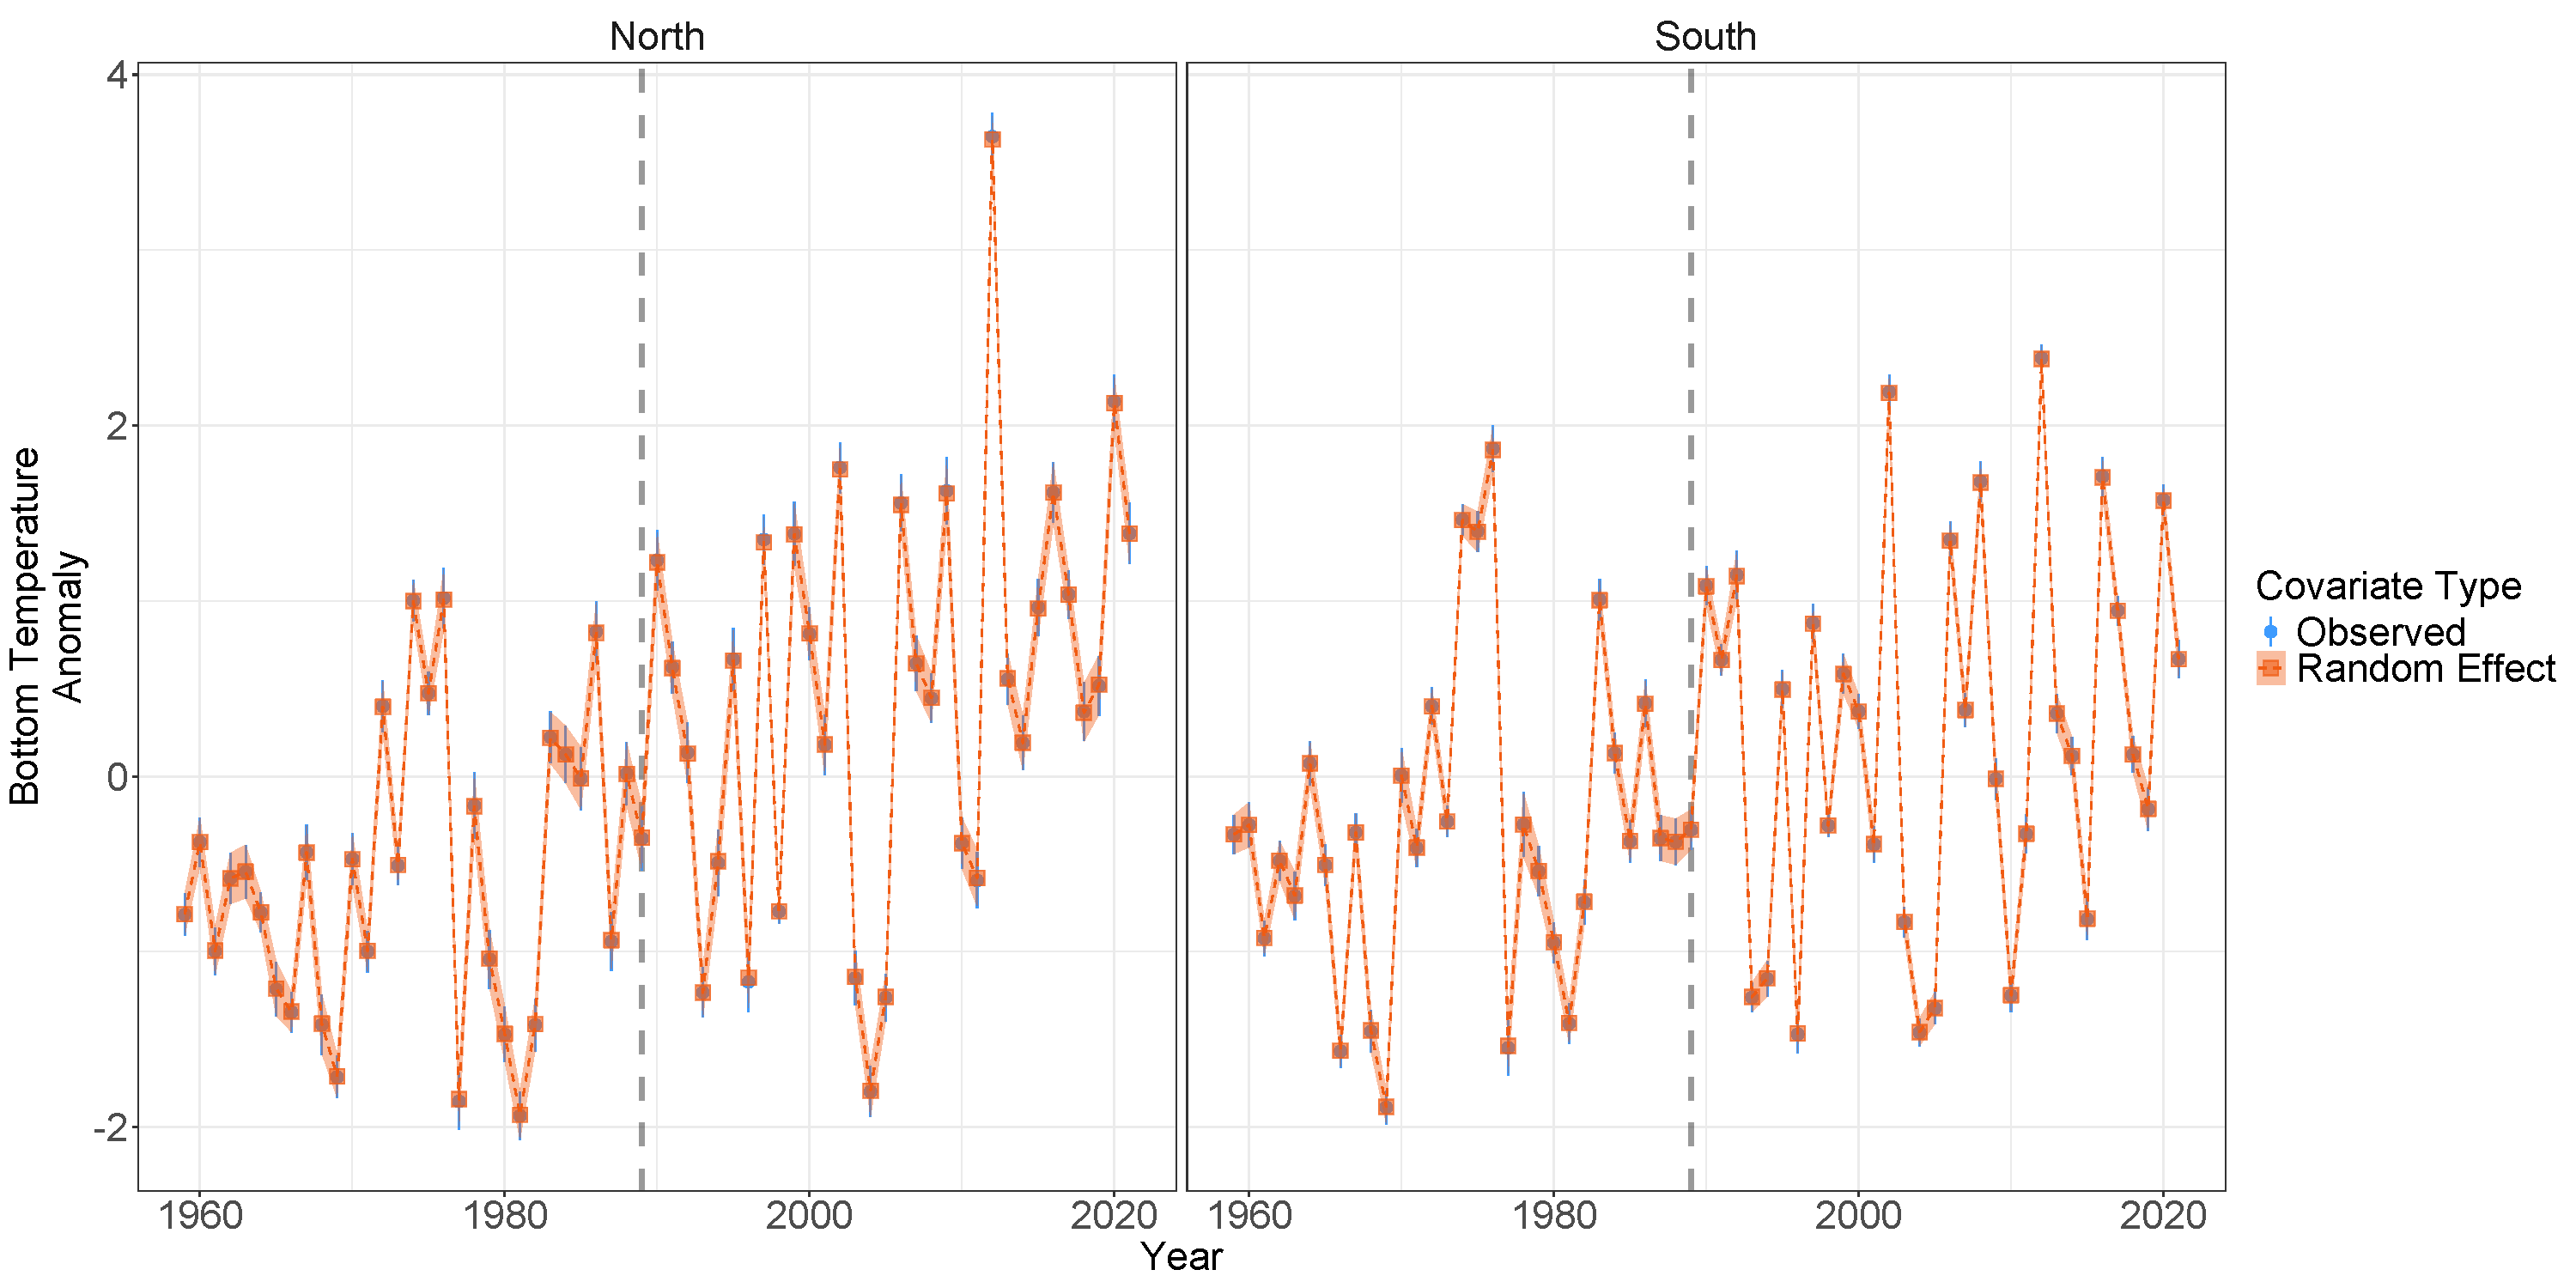
\includegraphics[width=1\linewidth]{BTA_full_fig} 

}

\caption{Observations with 95\% confidence intervals (points with vertical lines) and posterior estimates with 95\% confidence intervals (lines with polygons) of bottom temperature anomalies in the north and south regions from model $M_1$. Gray vertical line defines the first year that the black sea bass stock is modeled.}\label{fig:bottom-temperature}
\end{figure}
\end{landscape}
\pagebreak

\begin{figure}

{\centering 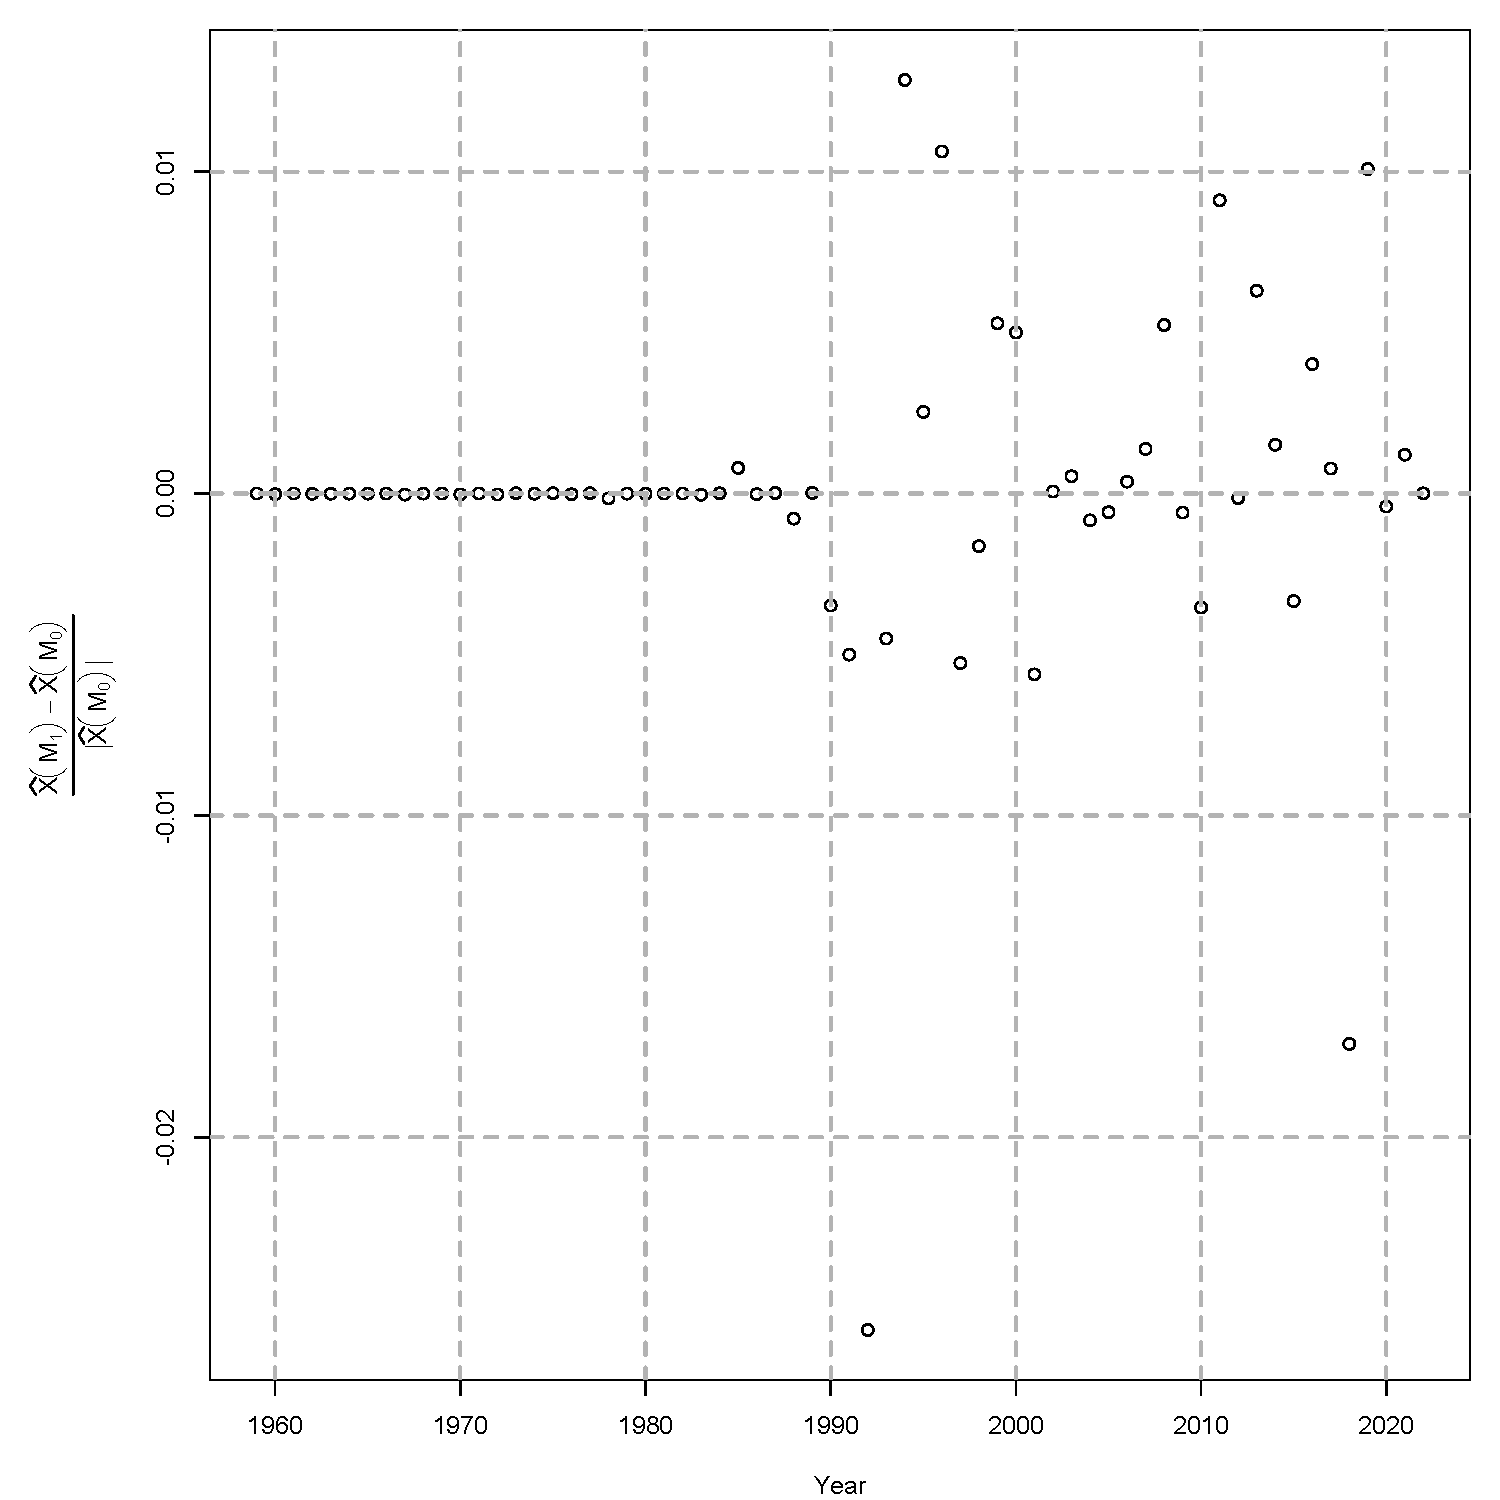
\includegraphics[height=0.95\textheight]{Ecov_M1_rel_M0} 

}

\caption{Relative differences in posterior estimates of northern region bottom temperature anomalies ($\widehat X$) from the null model without effects on recruitment ($M_0$) and with effects on the northern stock component ($M_1$).}\label{fig:Ecov-M1-rel-M0}
\end{figure}

\begin{figure}

{\centering 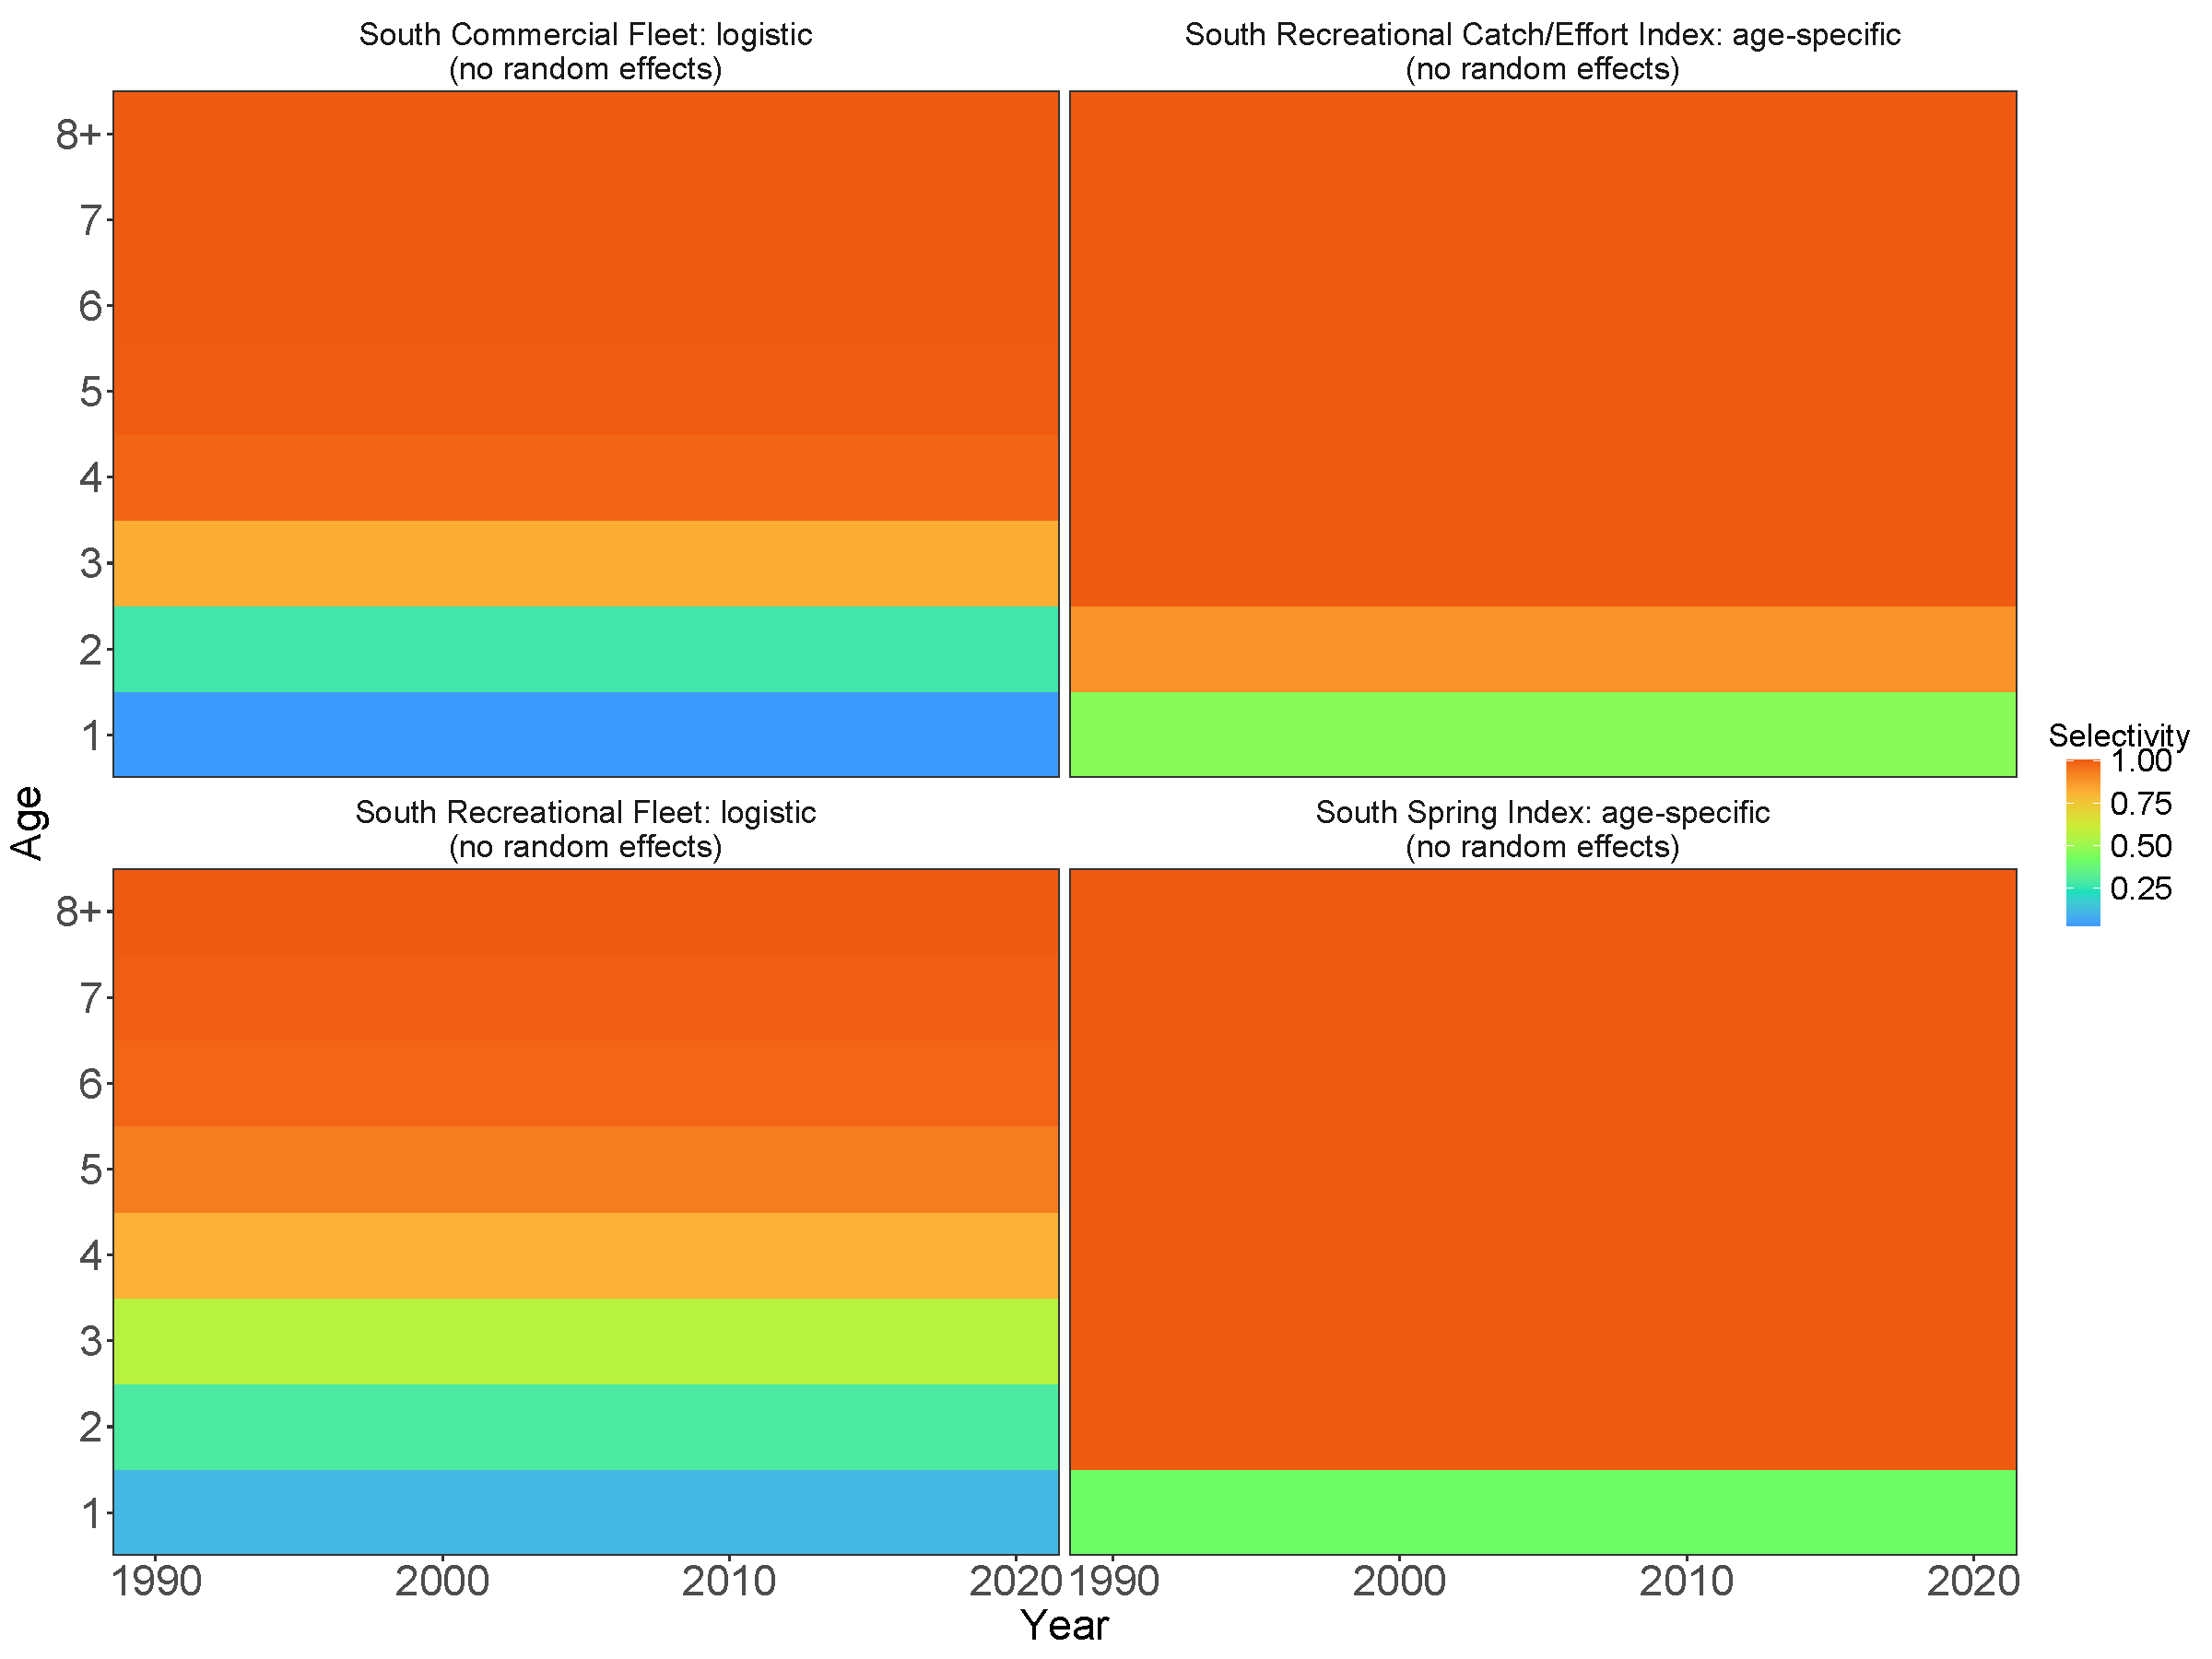
\includegraphics[height=0.95\textheight]{selectivity_south_plot} 

}

\caption{Selectivty for fleets and indices in the southern region.}\label{fig:selectivity-south}
\end{figure}

\begin{landscape}

\begin{figure}

{\centering 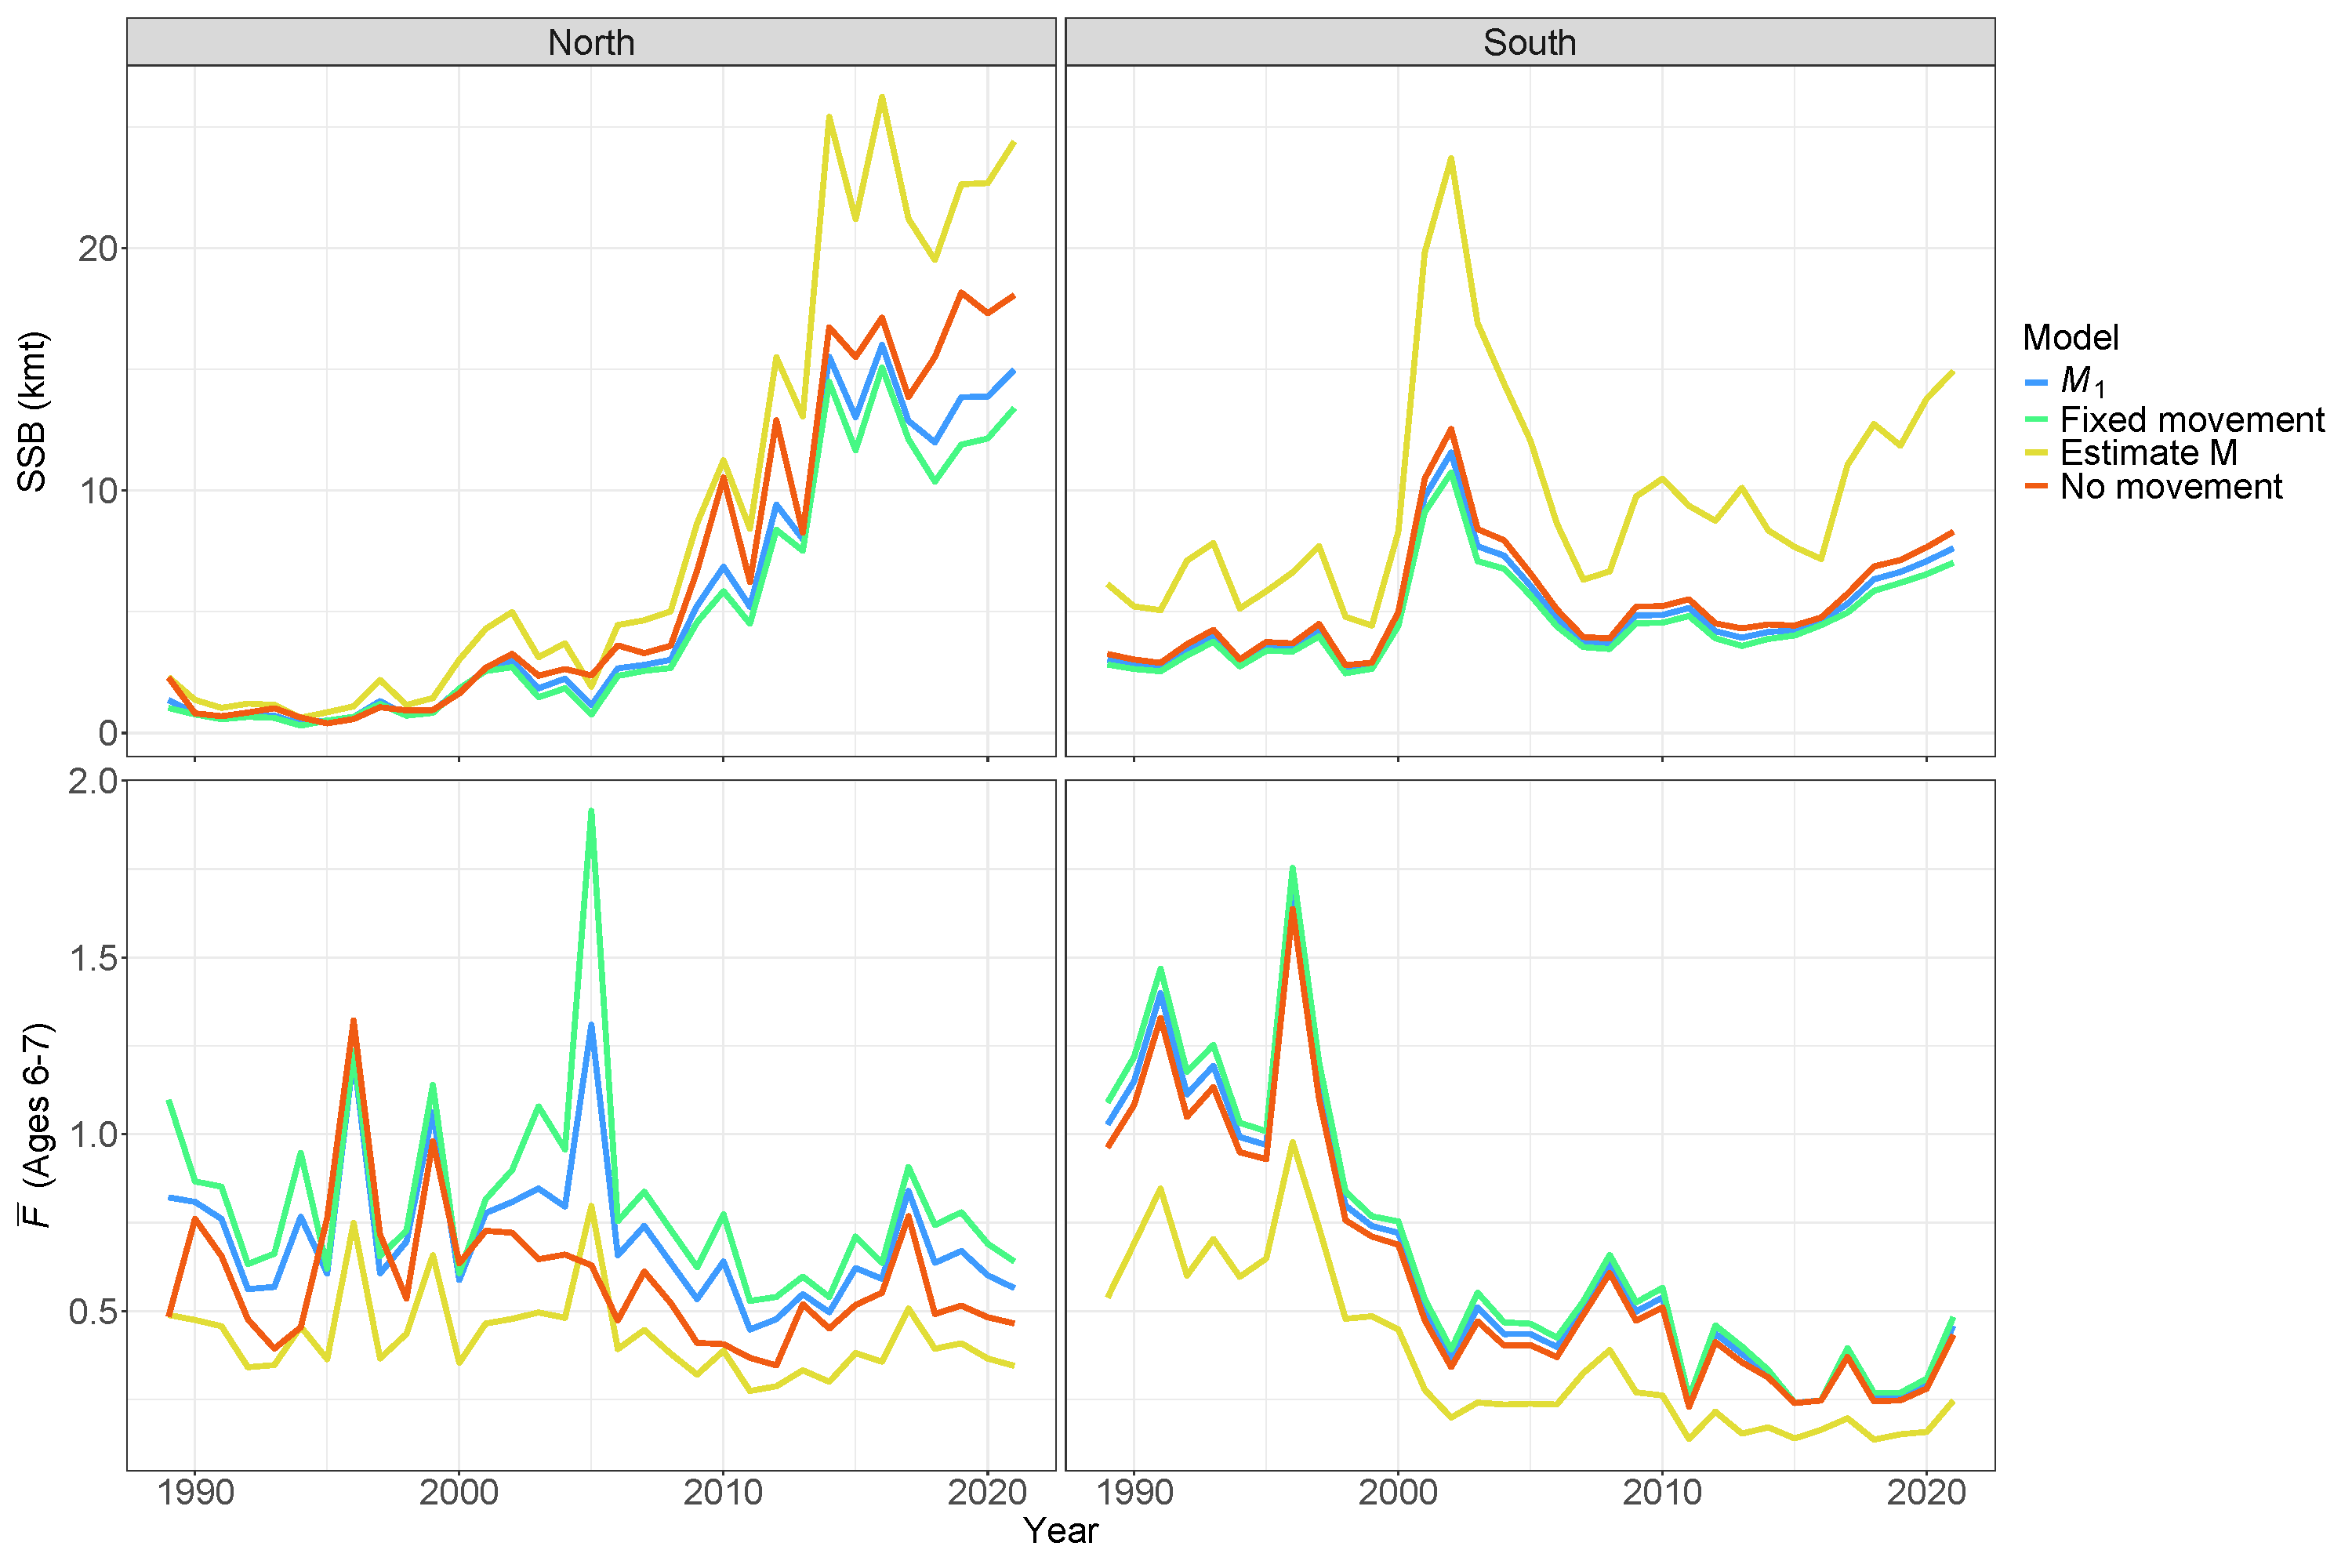
\includegraphics[height=0.95\textheight]{SSB_F_sensitivity_plots} 

}

\caption{Estimates of annual SSB and fishing mortality rates for the best performing model $M_1$ and models that are otherwise the same except where  1) movement rates are fixed at the means for the prior distribution, 2) a constant natural mortality rate is estimated, or 3) there is no movement for either stock component.}\label{fig:sensitivity-plots}
\end{figure}
\end{landscape}

\begin{figure}

{\centering 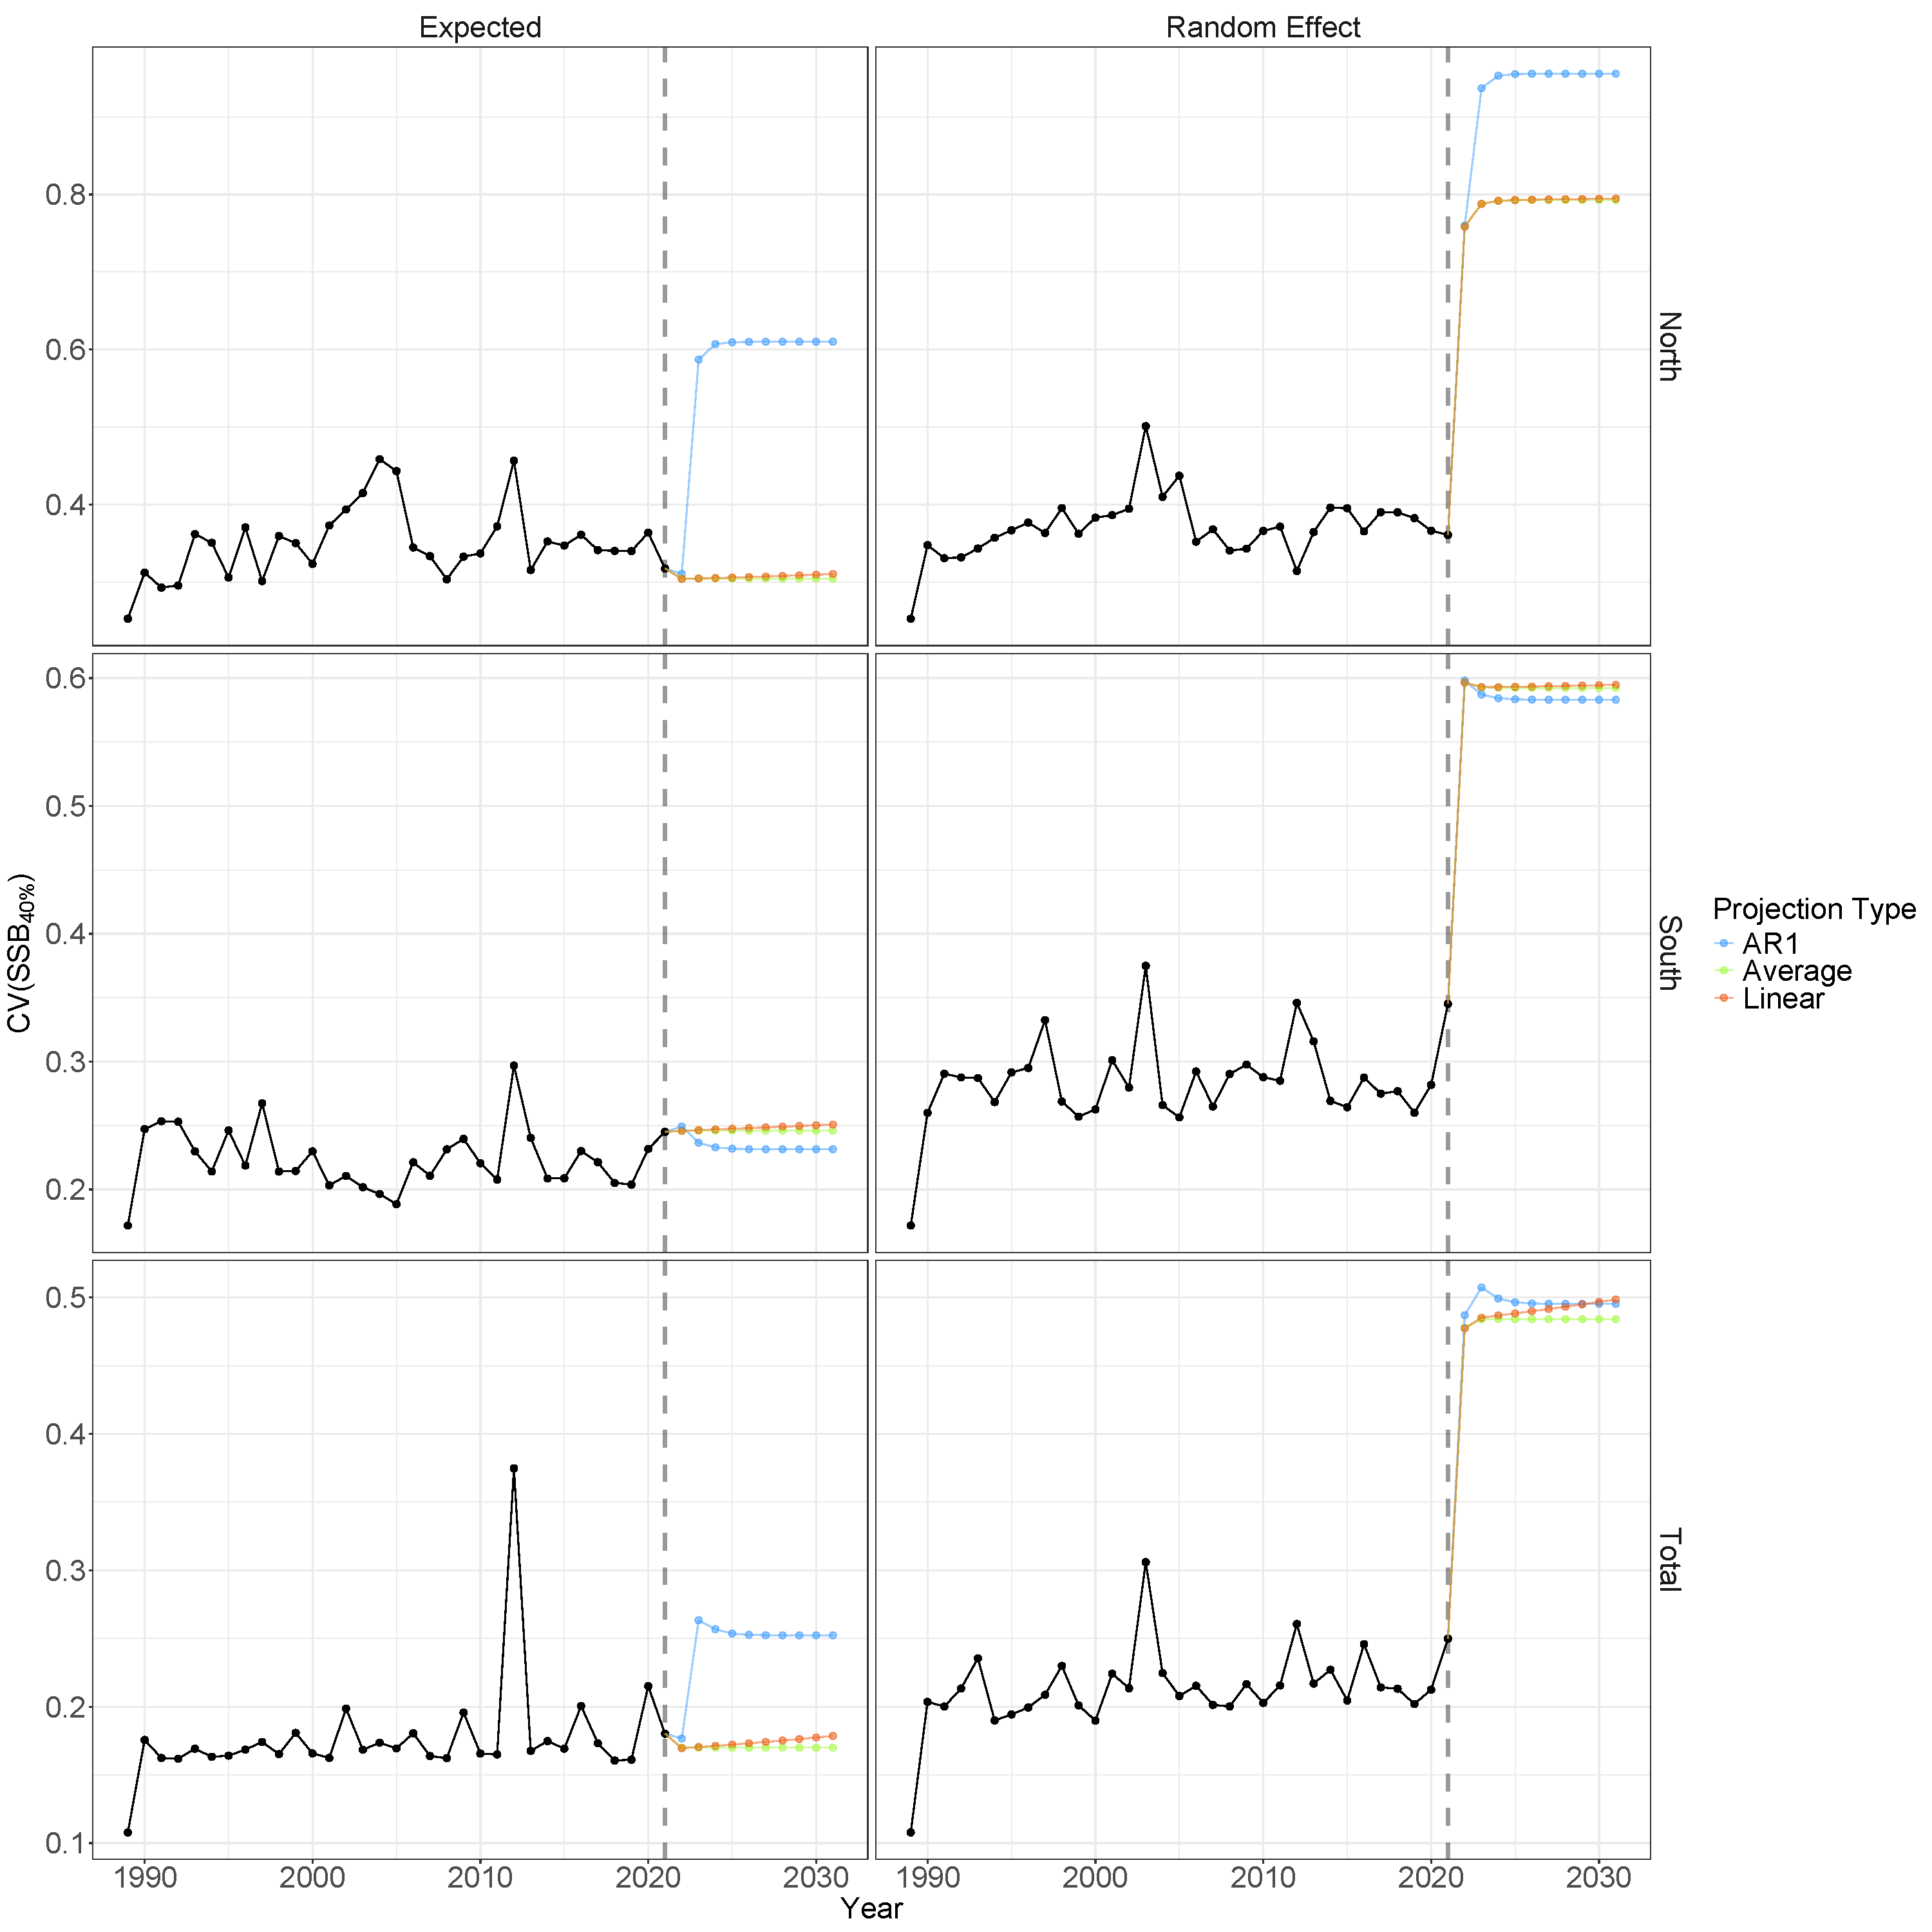
\includegraphics[height=0.95\textheight]{proj_SSB40_CV} 

}

\caption{Coefficients of variation for annual equilibrium SSB$_{40\%}$ as a function of annual expected recruitment or recruitment random effects and annual inputs to $\upphi(\widetilde{F})$ calculations and alternative annual recruitment types. Estimates in years after 2021 are from projecting model $M_1$ under three alternative assumptions for the bottom temperature anomolies. Vertical dotted lines indicate the last year of data.}\label{fig:annual-SSB40-cvs}
\end{figure}
\begin{figure}

{\centering 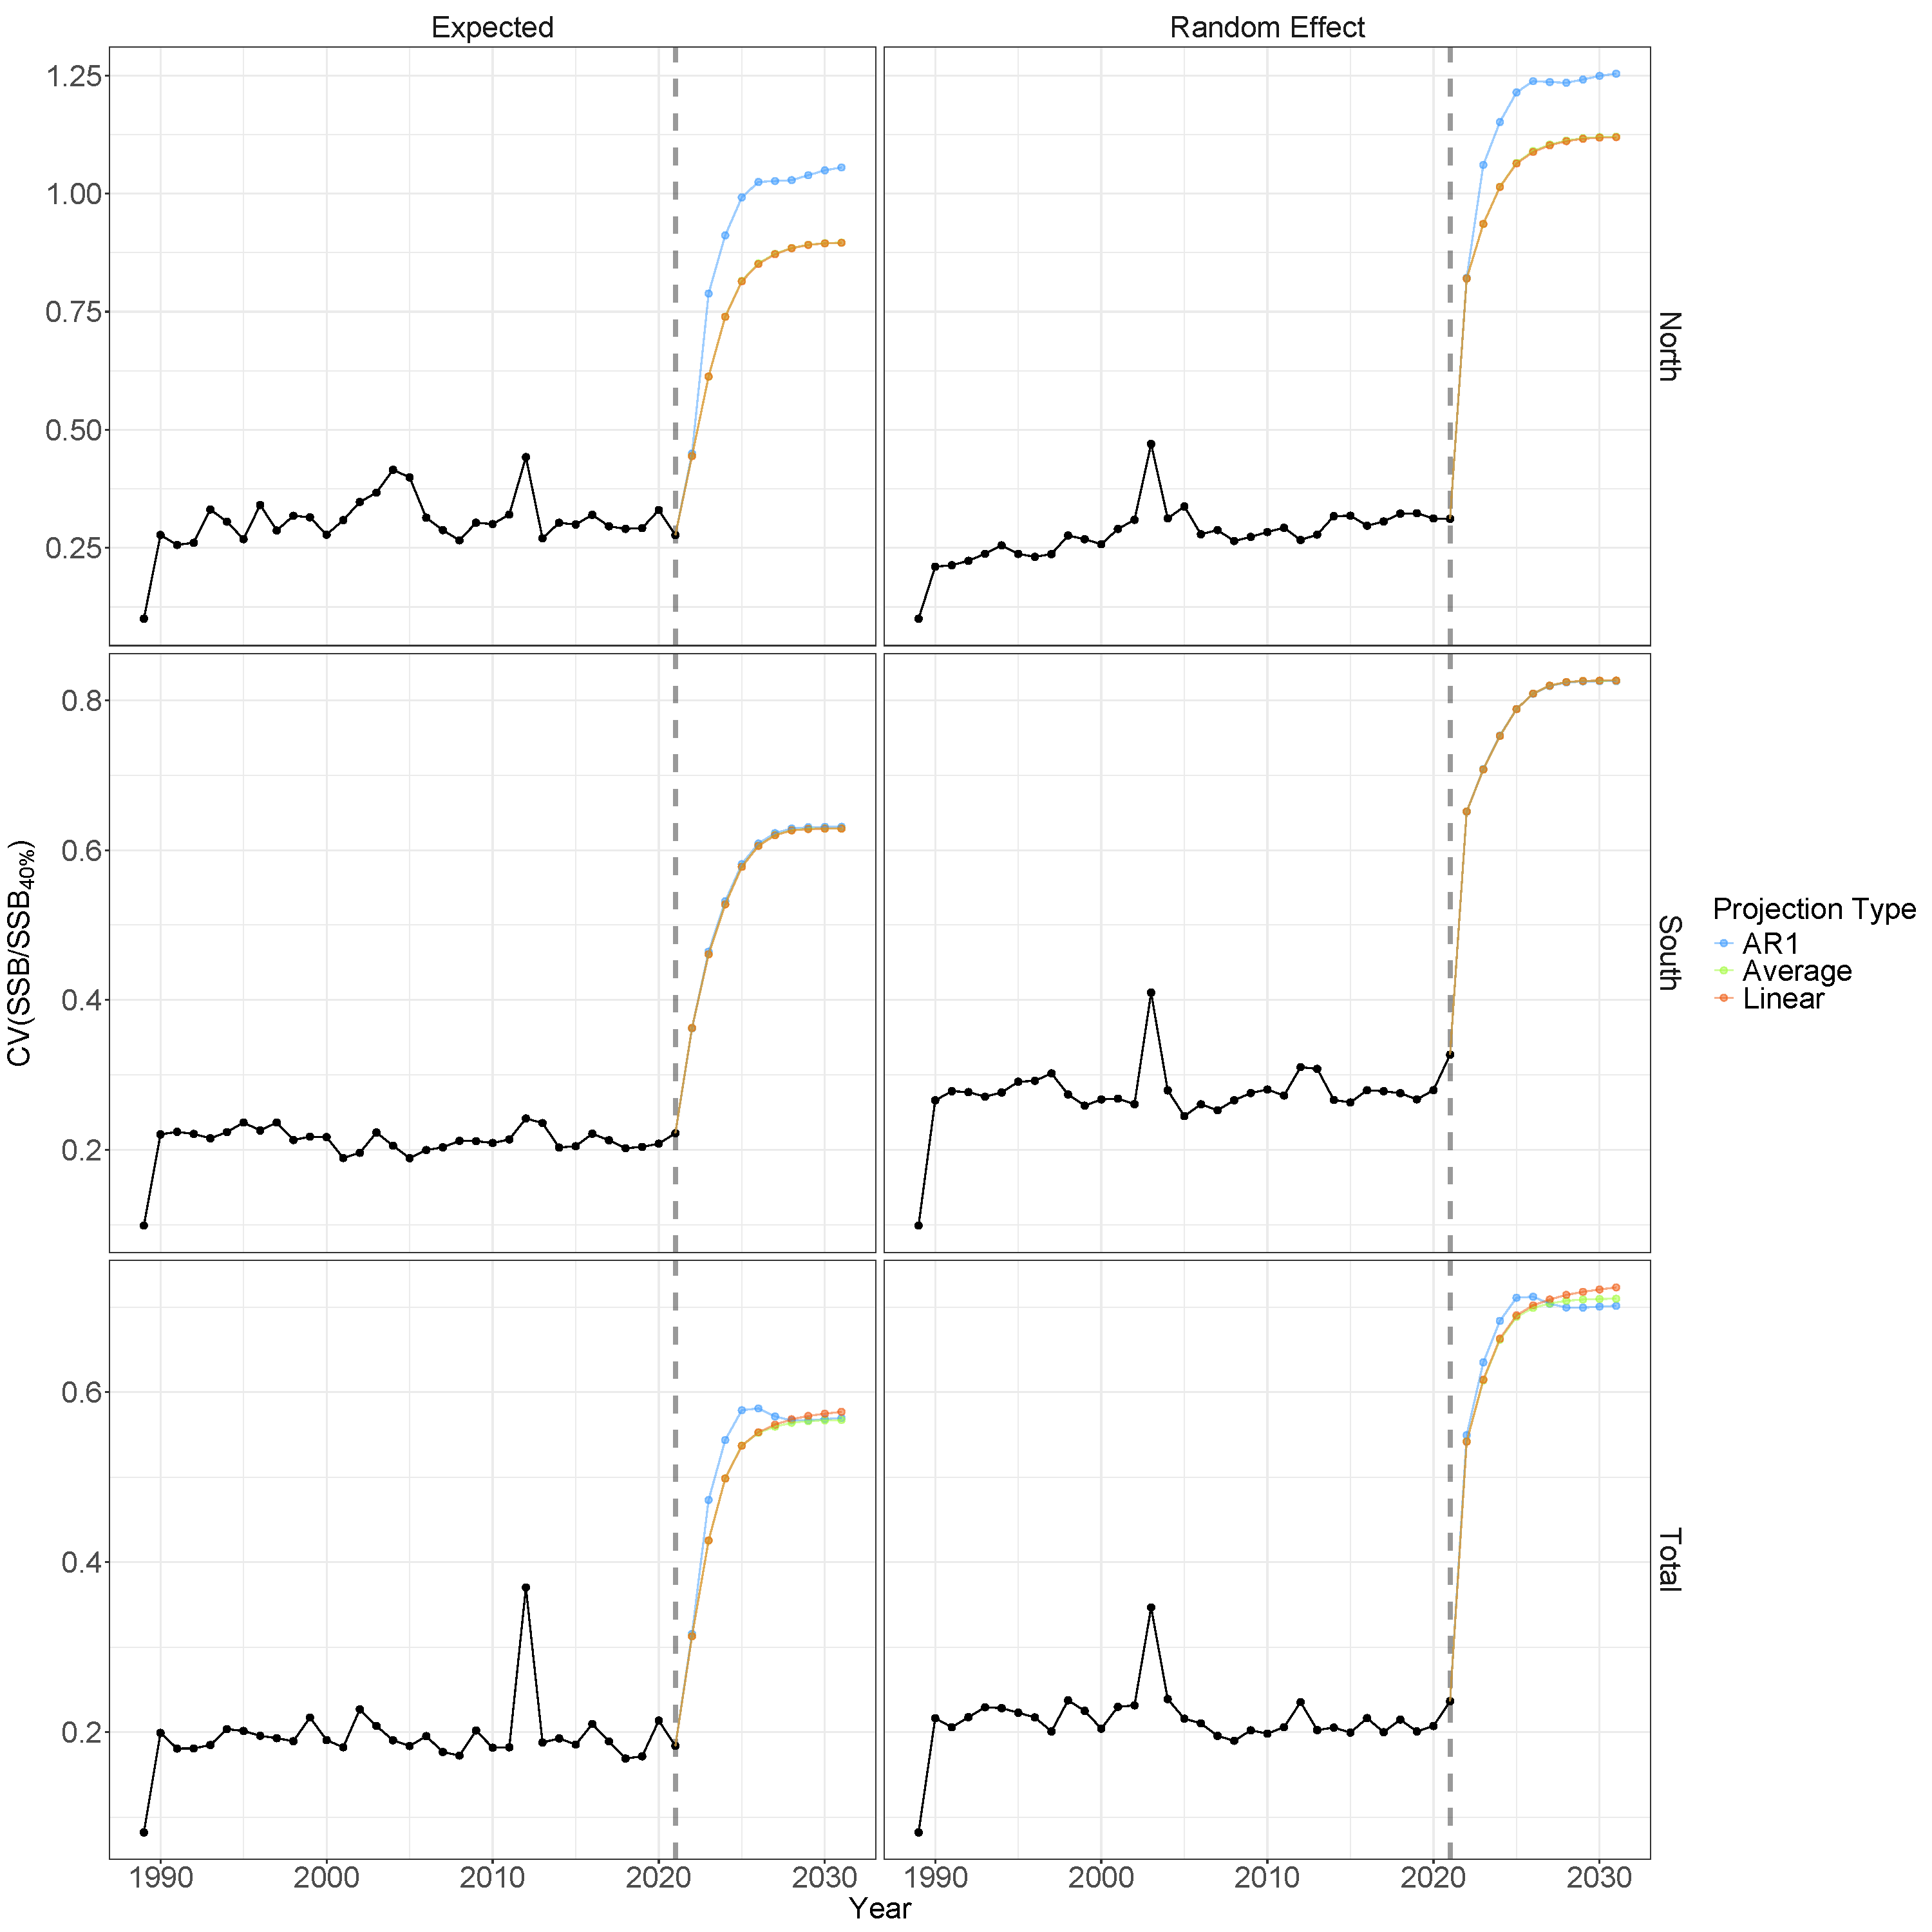
\includegraphics[height=0.95\textheight]{proj_SSB_status_CV} 

}

\caption{Coefficients of variation for annual ratios of SSB and equilibrium SSB$_{40\%}$ where the latter is a function of annual expected recruitment or recruitment random effects and annual inputs to $\upphi(\widetilde{F})$ calculations. Estimates in years after 2021 are from projecting model $M_1$ under three alternative assumptions for the bottom temperature anomolies. Vertical dotted lines indicate the last year of data.}\label{fig:annual-SSB-status-cvs}
\end{figure}

\begin{figure}

{\centering 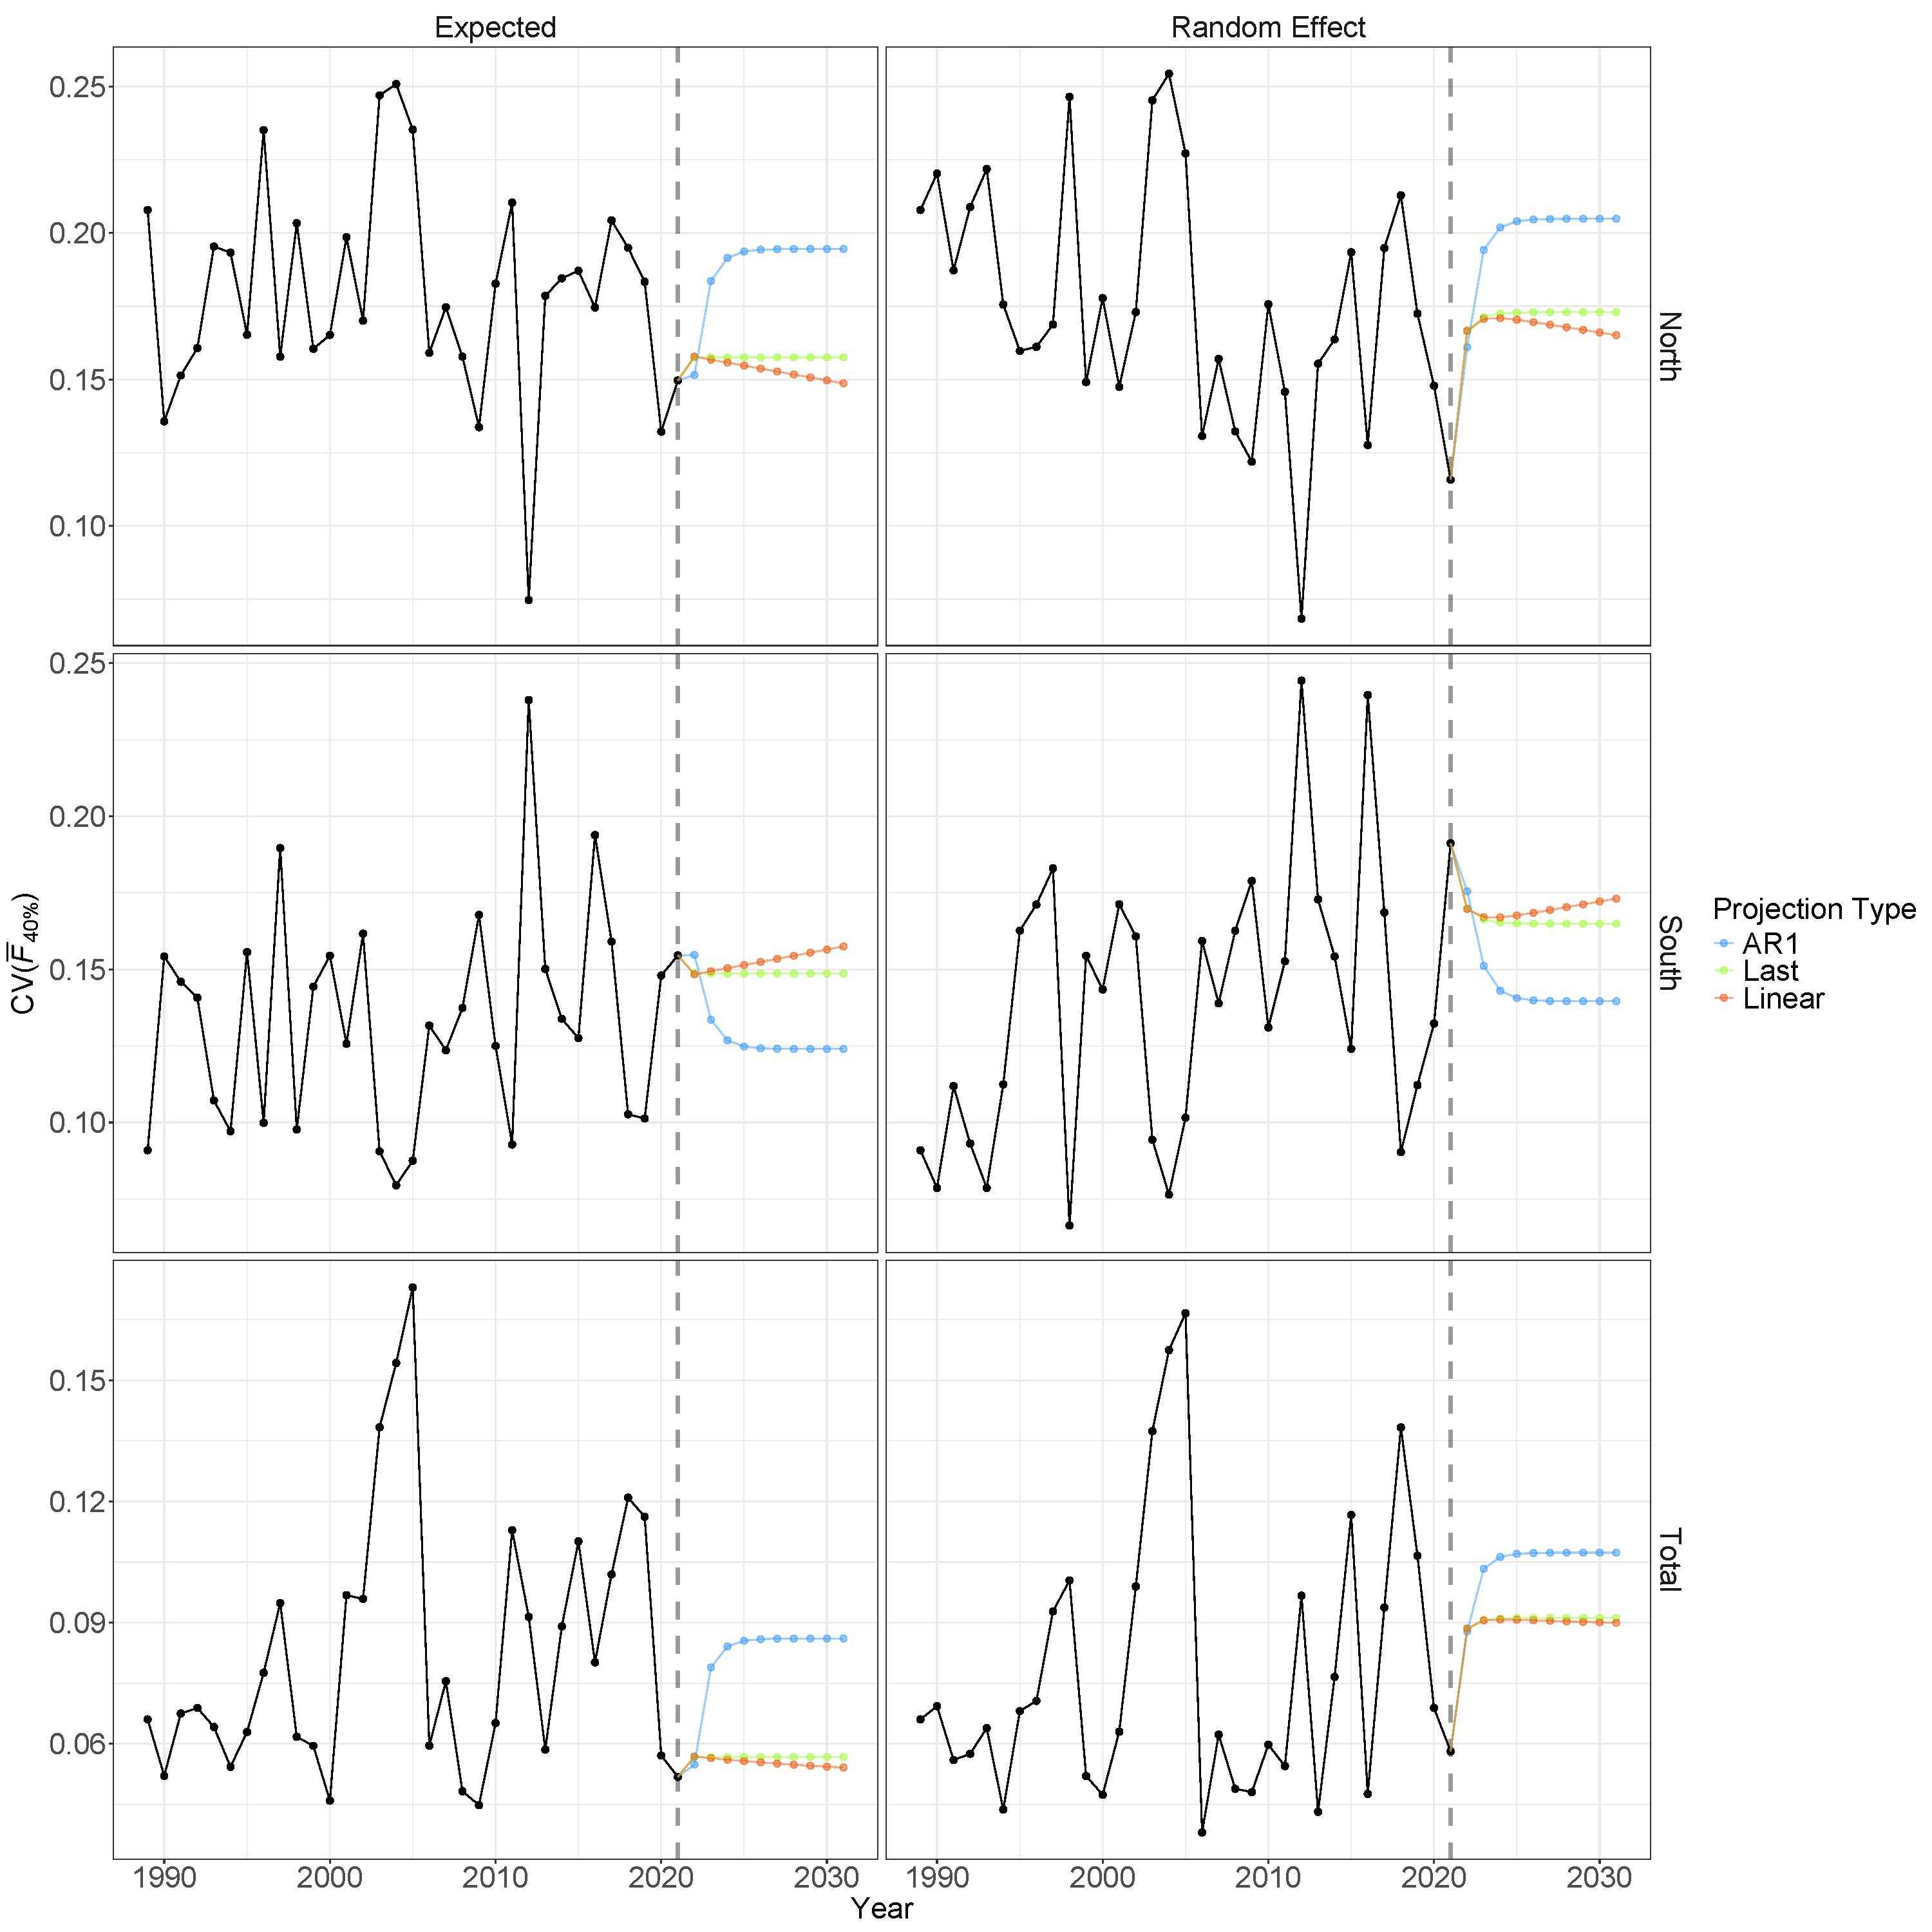
\includegraphics[height=0.95\textheight]{proj_F40_CV} 

}

\caption{Coefficients of variation for annual equilibrium average $F$ at ages 6 and 7 that produces the 40\% spawning potential ratio as a function of annual expected recruitment or recruitment random effects and annual inputs to $\upphi(\widetilde{F})$ calculations. Estimates in years after 2021 are from projecting model $M_1$ under three alternative assumptions for the bottom temperature anomolies. Vertical dotted lines indicate the last year of data.}\label{fig:annual-F40-cvs}
\end{figure}

\begin{figure}

{\centering 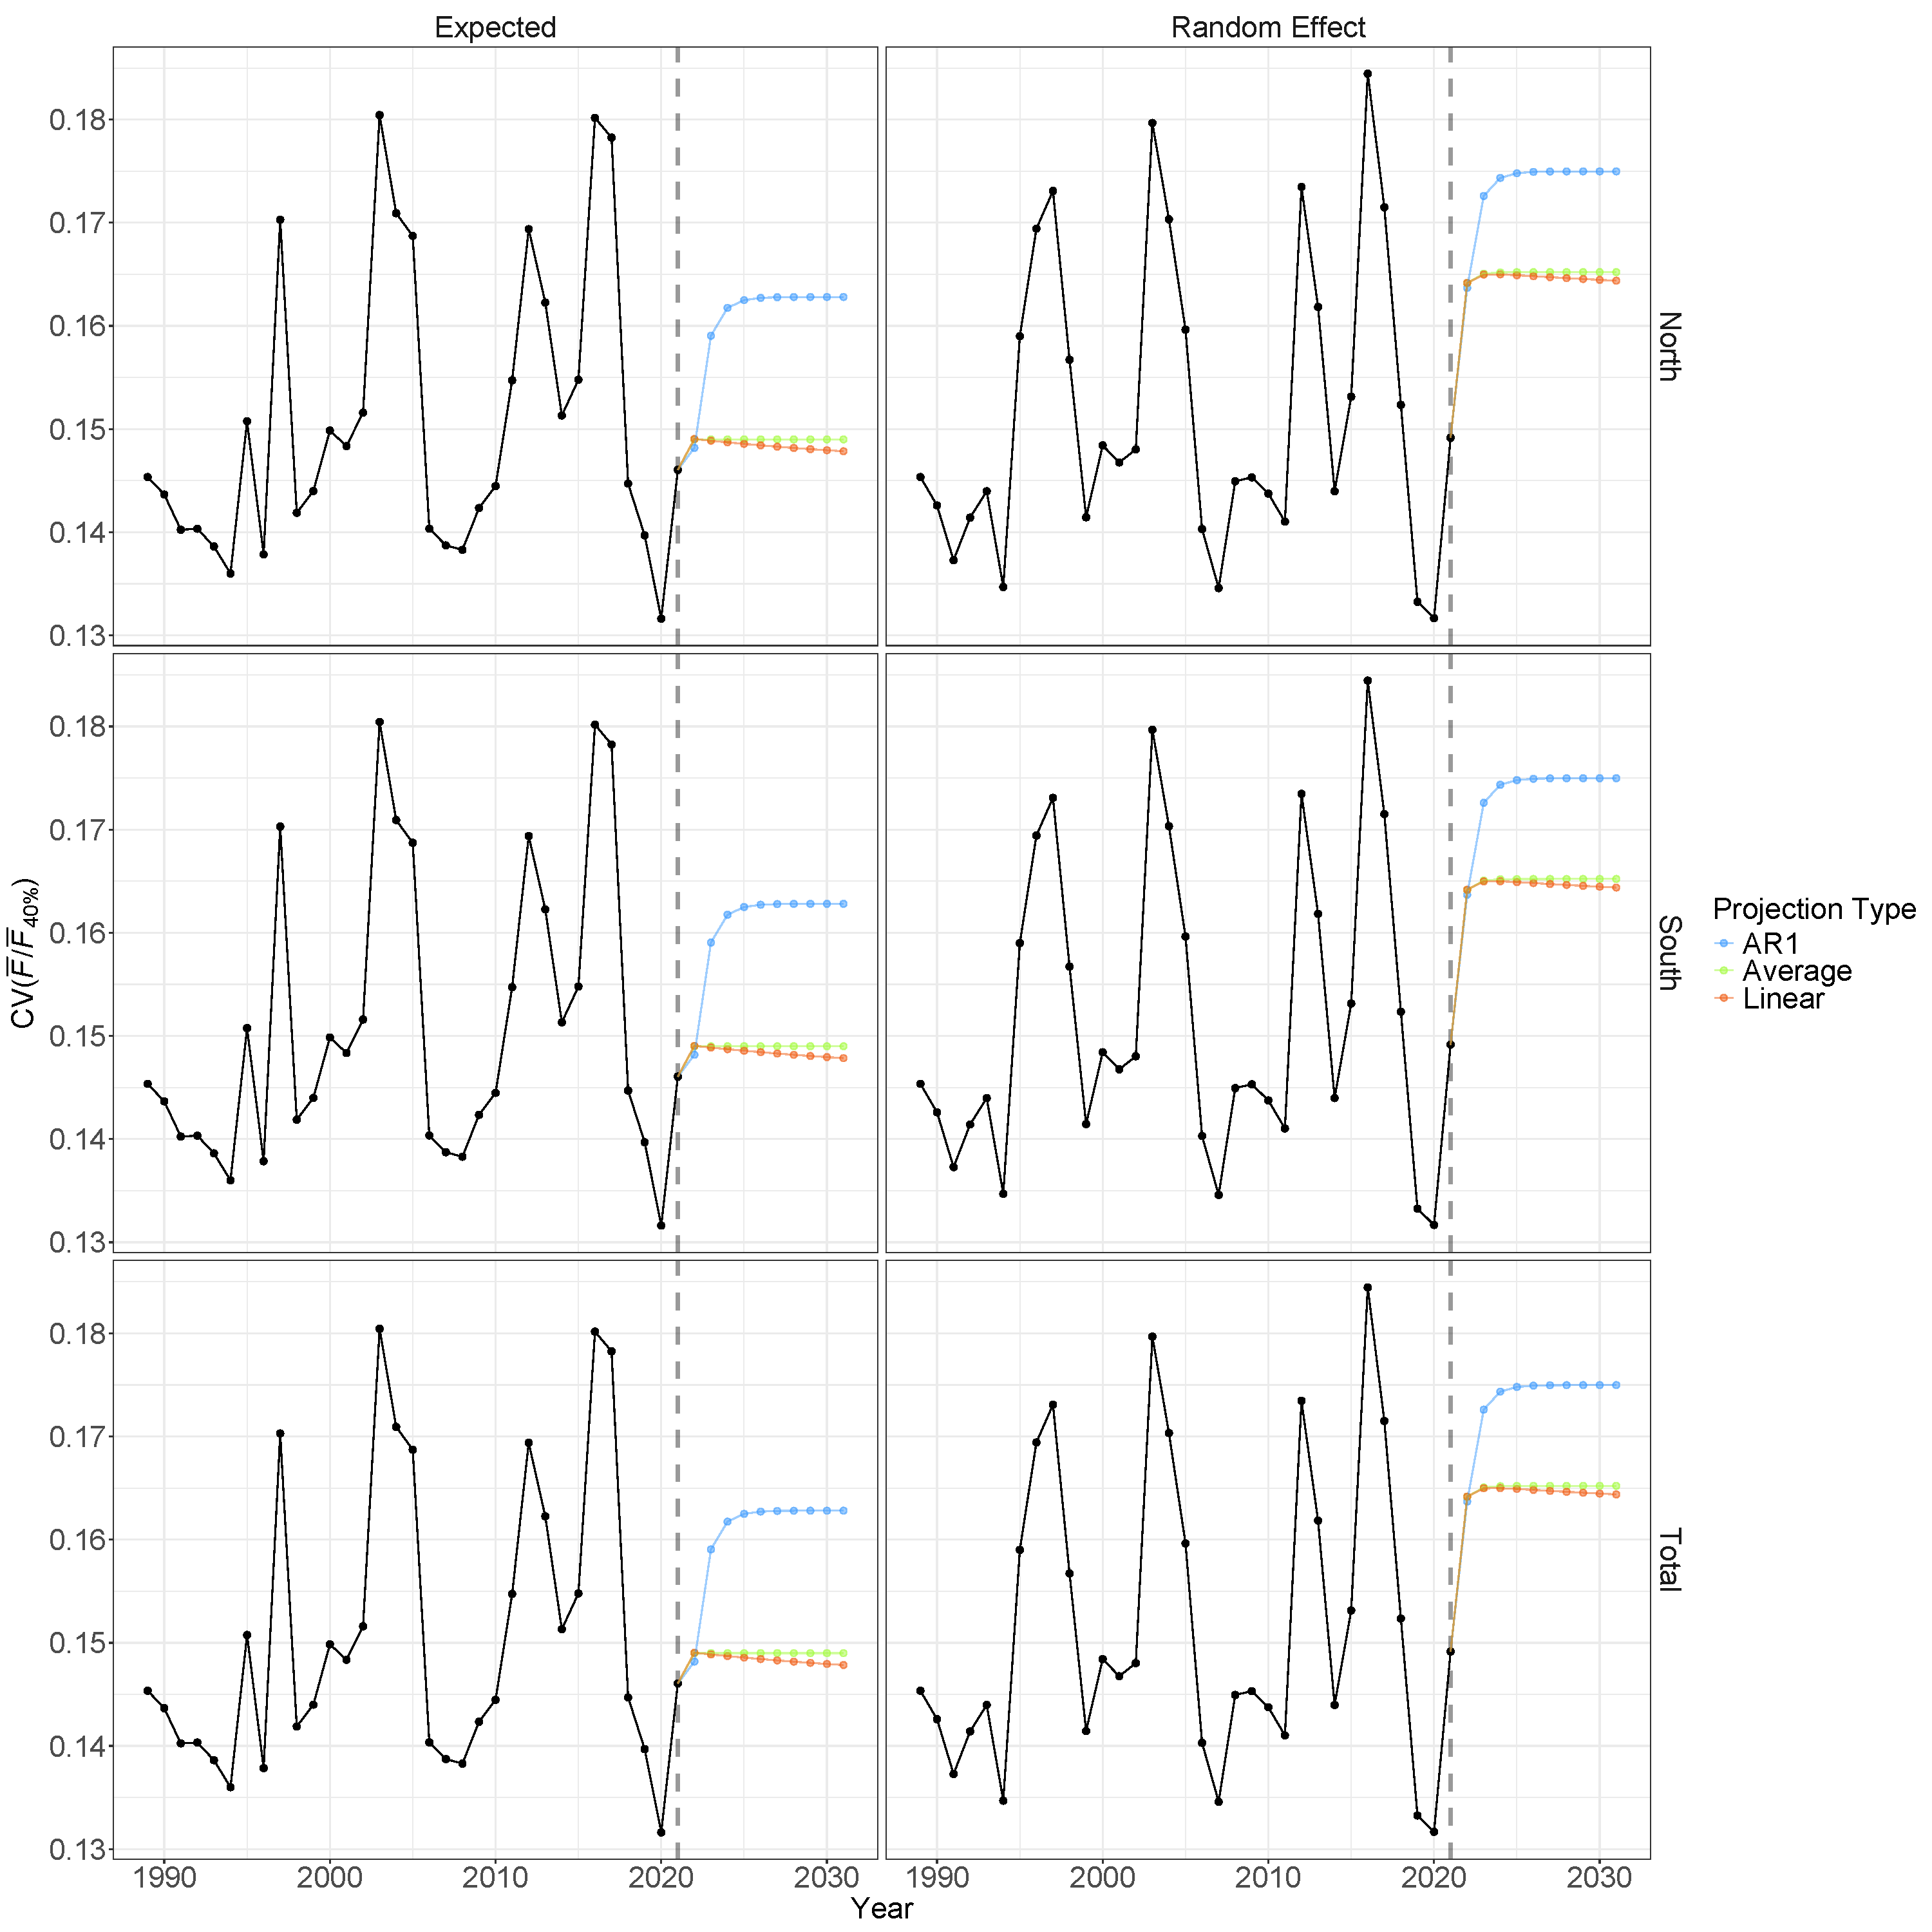
\includegraphics[height=0.95\textheight]{proj_F_status_CV} 

}

\caption{Coefficients of variation for annual ratios of average fishing mortality and equilibrium $\bar{F}_{40\%}$ at ages 6 and 7 where the latter is a function of annual expected recruitment or recruitment random effects and annual inputs to $\upphi(\widetilde{F})$ calculations. Estimates in years after 2021 are from projecting model $M_1$ under three alternative assumptions for the bottom temperature anomolies. Vertical dotted lines indicate the last year of data.}\label{fig:annual-F-status-cvs}
\end{figure}

\begin{landscape}

\begin{figure}

{\centering 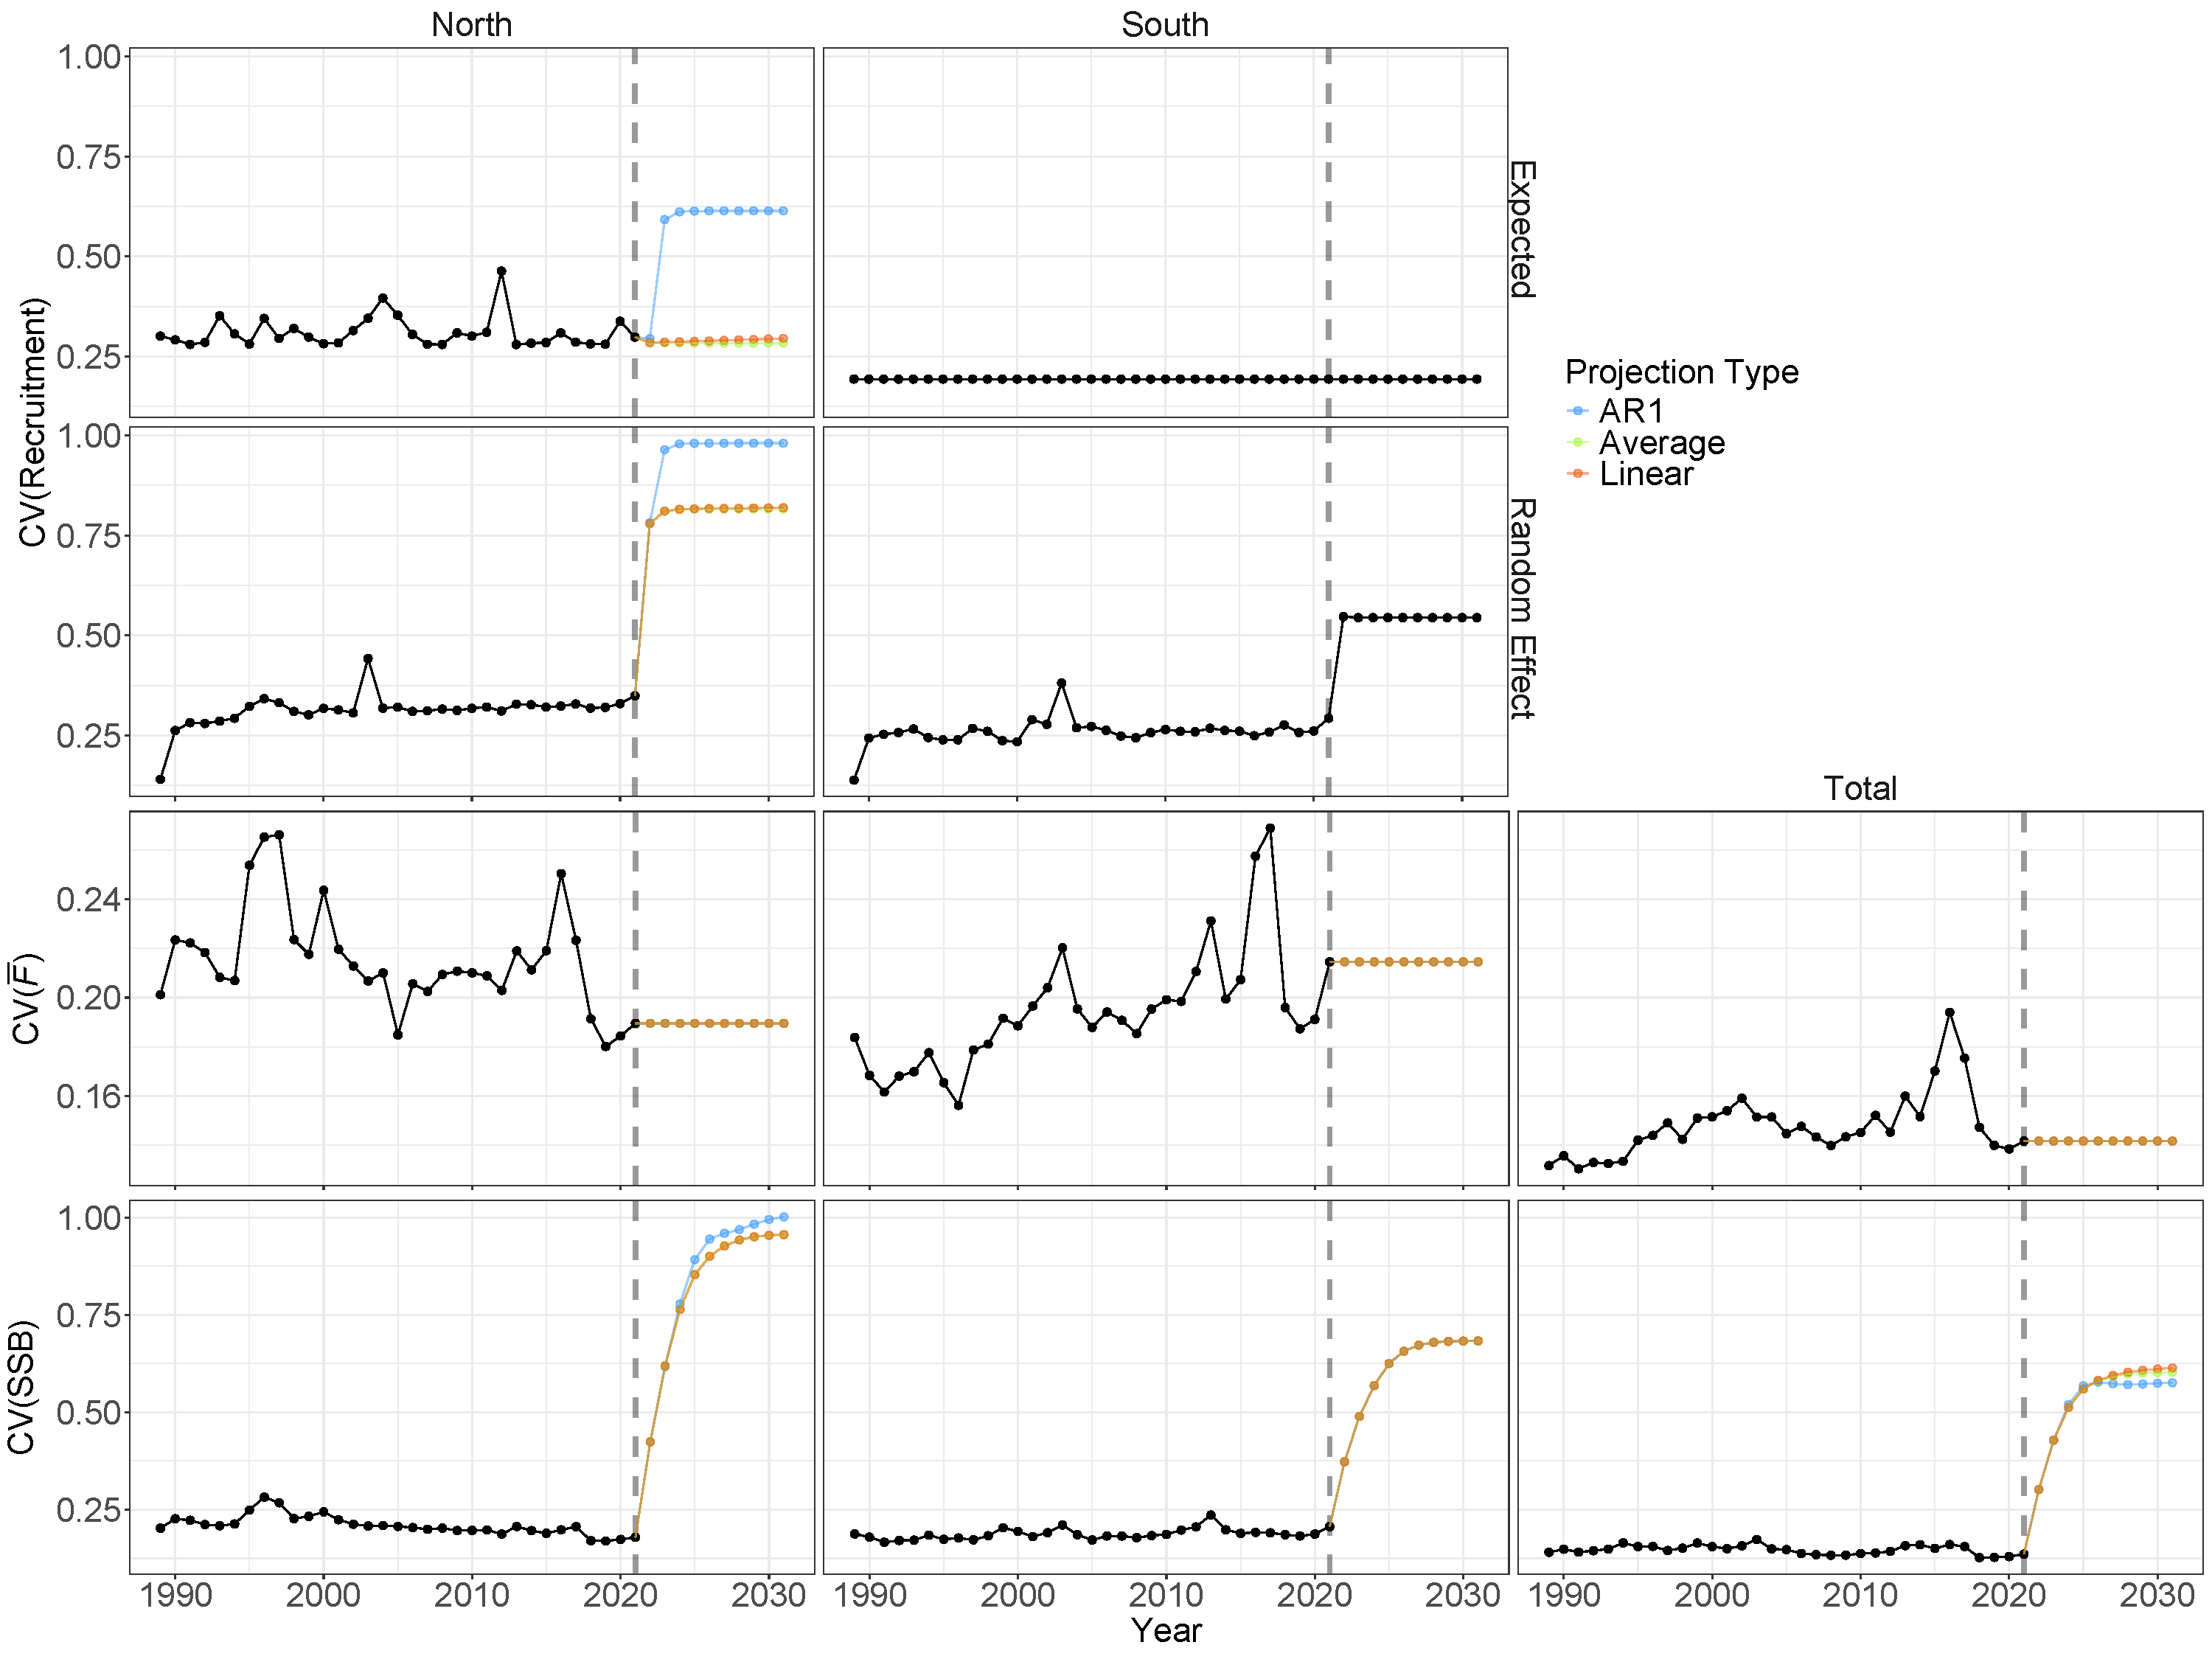
\includegraphics[height=0.9\textheight]{R_SSB_F_cv_results} 

}

\caption{Coefficients of variation for estimates of alternative recruitment estimates (random effects or expected), average fishing mortality at age 6 and 7, and SSB by region and in total from model $M_1$. Values in years after 2021 are from projecting model $M_1$ under three alternative assumptions for the bottom temperature anomolies. Vertical dotted lines indicate the last year of data.}\label{fig:R-F-SSB-CVs}
\end{figure}
\end{landscape}

\pagebreak

\begin{figure}

{\centering 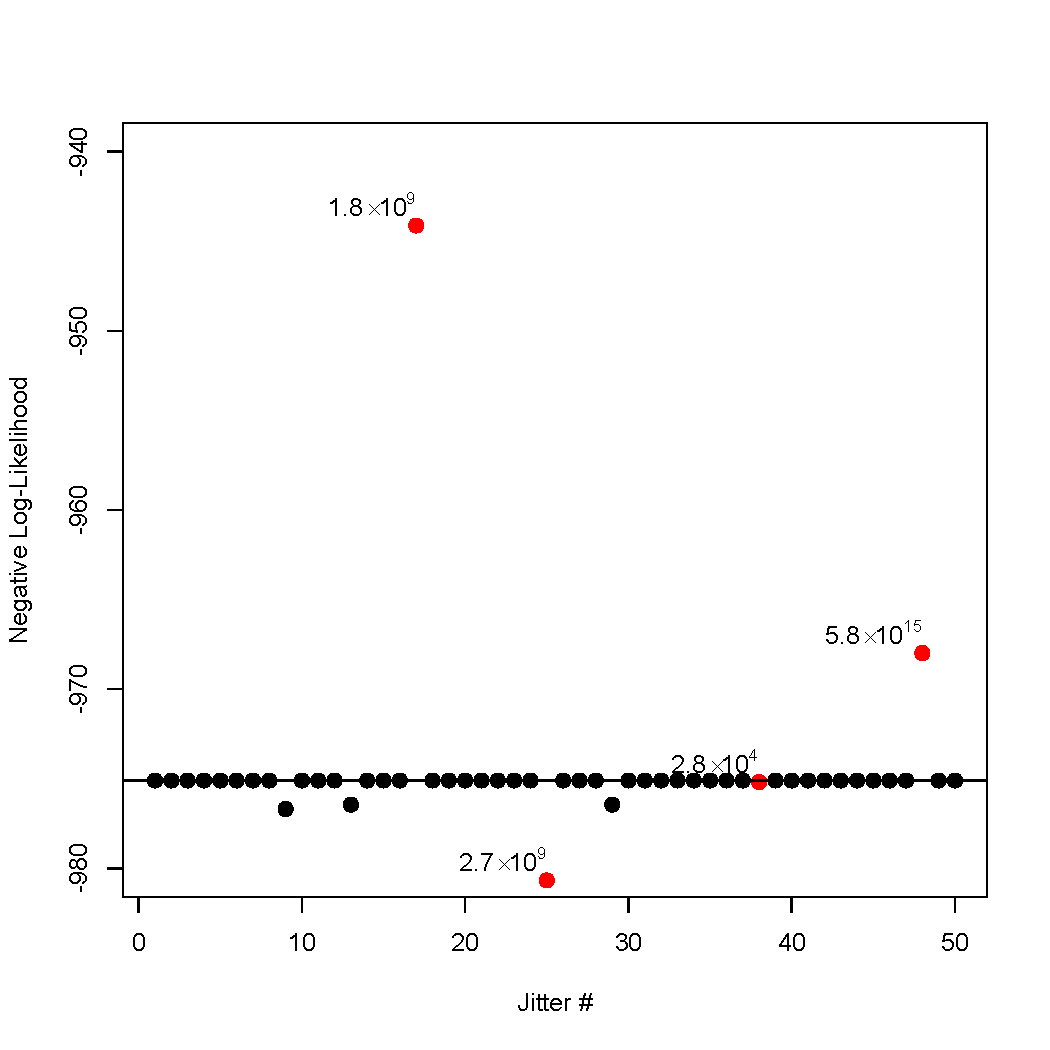
\includegraphics[width=1\linewidth]{fit_0_jitter_plt} 

}

\caption{Minimized negative log-likelihood for 50 fits where minimization used initial parameter values jittered from those provided by an initial fit for model $M_0$. Black jitters had maximum absolute gradient values < $10^{-2}$ and red jitters had values > 1.}\label{fig:jitter-M0}
\end{figure}
\pagebreak

\begin{figure}

{\centering 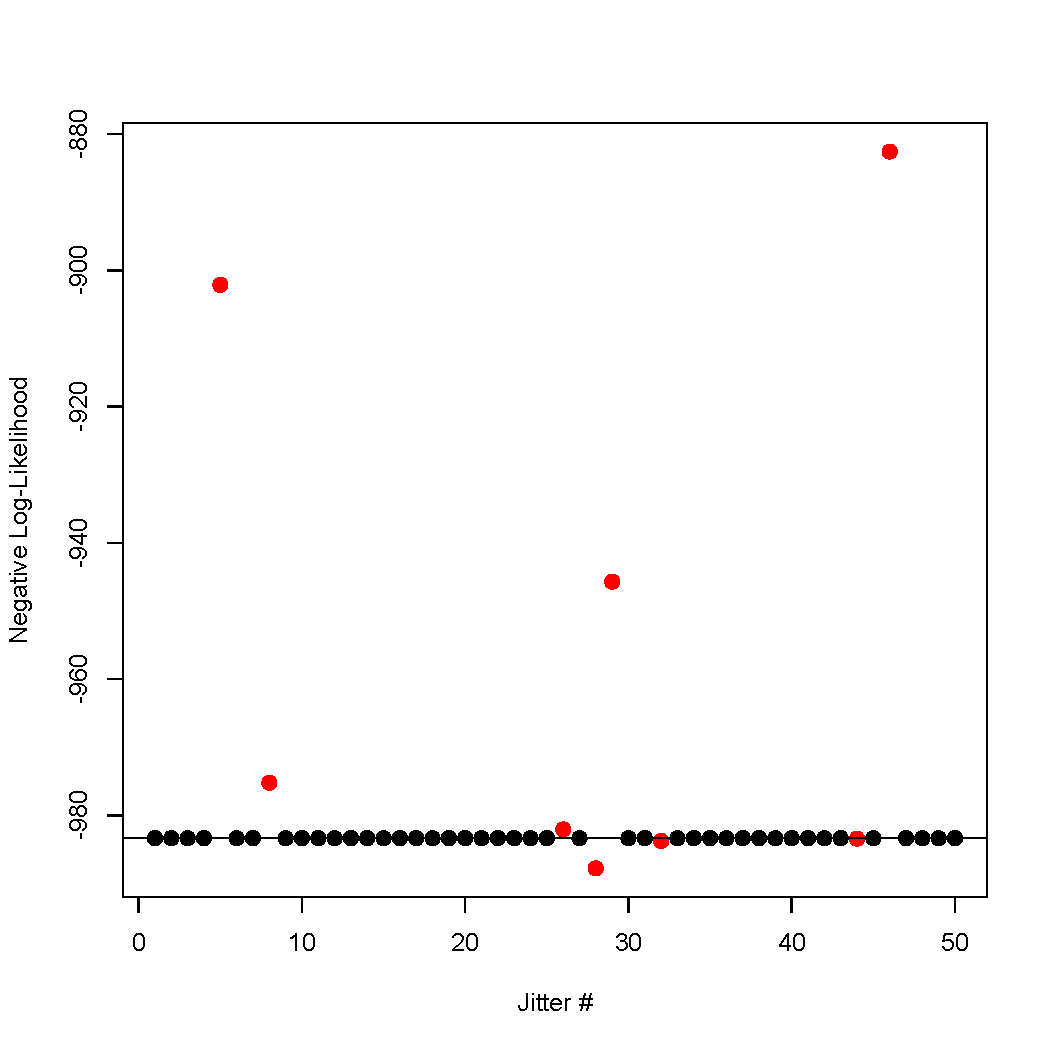
\includegraphics[width=1\linewidth]{fit_1_jitter_plt} 

}

\caption{Minimized negative log-likelihood for 50 fits where minimization used initial parameter values jittered from those provided by an initial fit for model $M_1$. Fits with black dots had maximum absolute gradient value < 0.01 and fits with red dots had values > 10.}\label{fig:jitter-M1}
\end{figure}
\pagebreak

\begin{figure}

{\centering 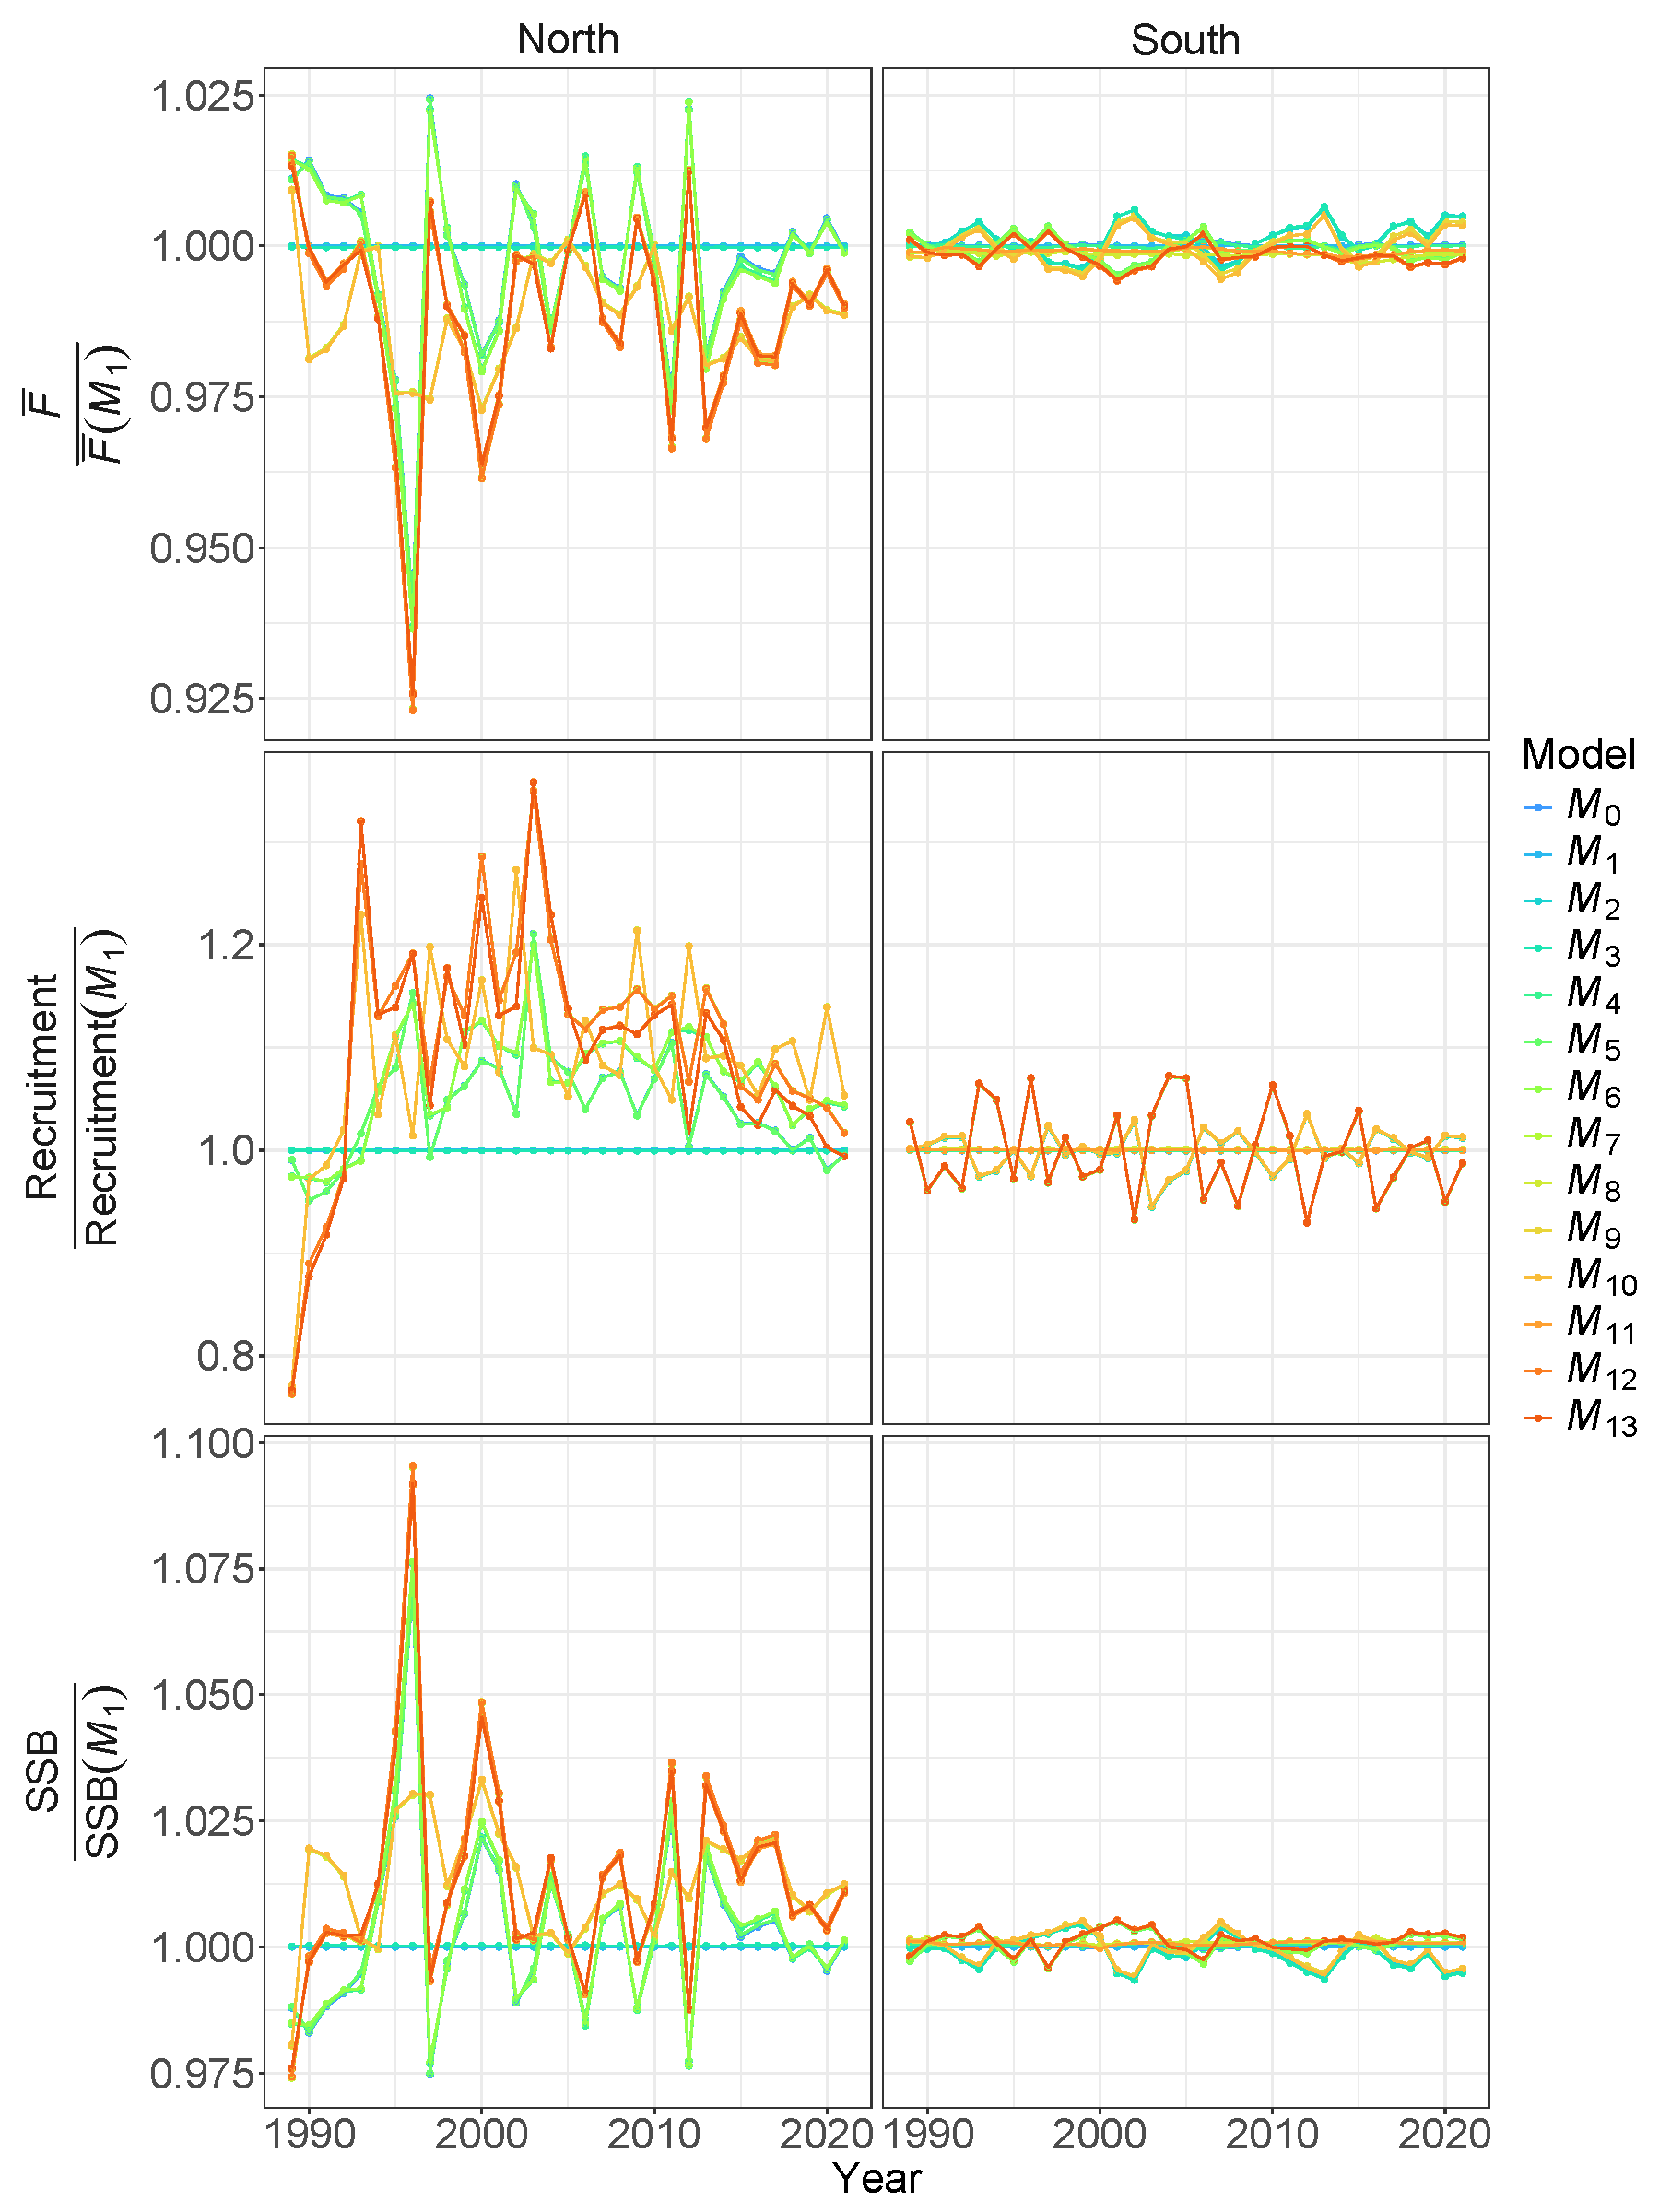
\includegraphics[height=0.95\textheight]{SSB_F_R_rel_M1} 

}

\caption{Estimates of SSB, F, and recruitment relative to those of the best performing model, $M_1$.}\label{fig:SSB-F-R-rel-M1}
\end{figure}

\begin{figure}

{\centering 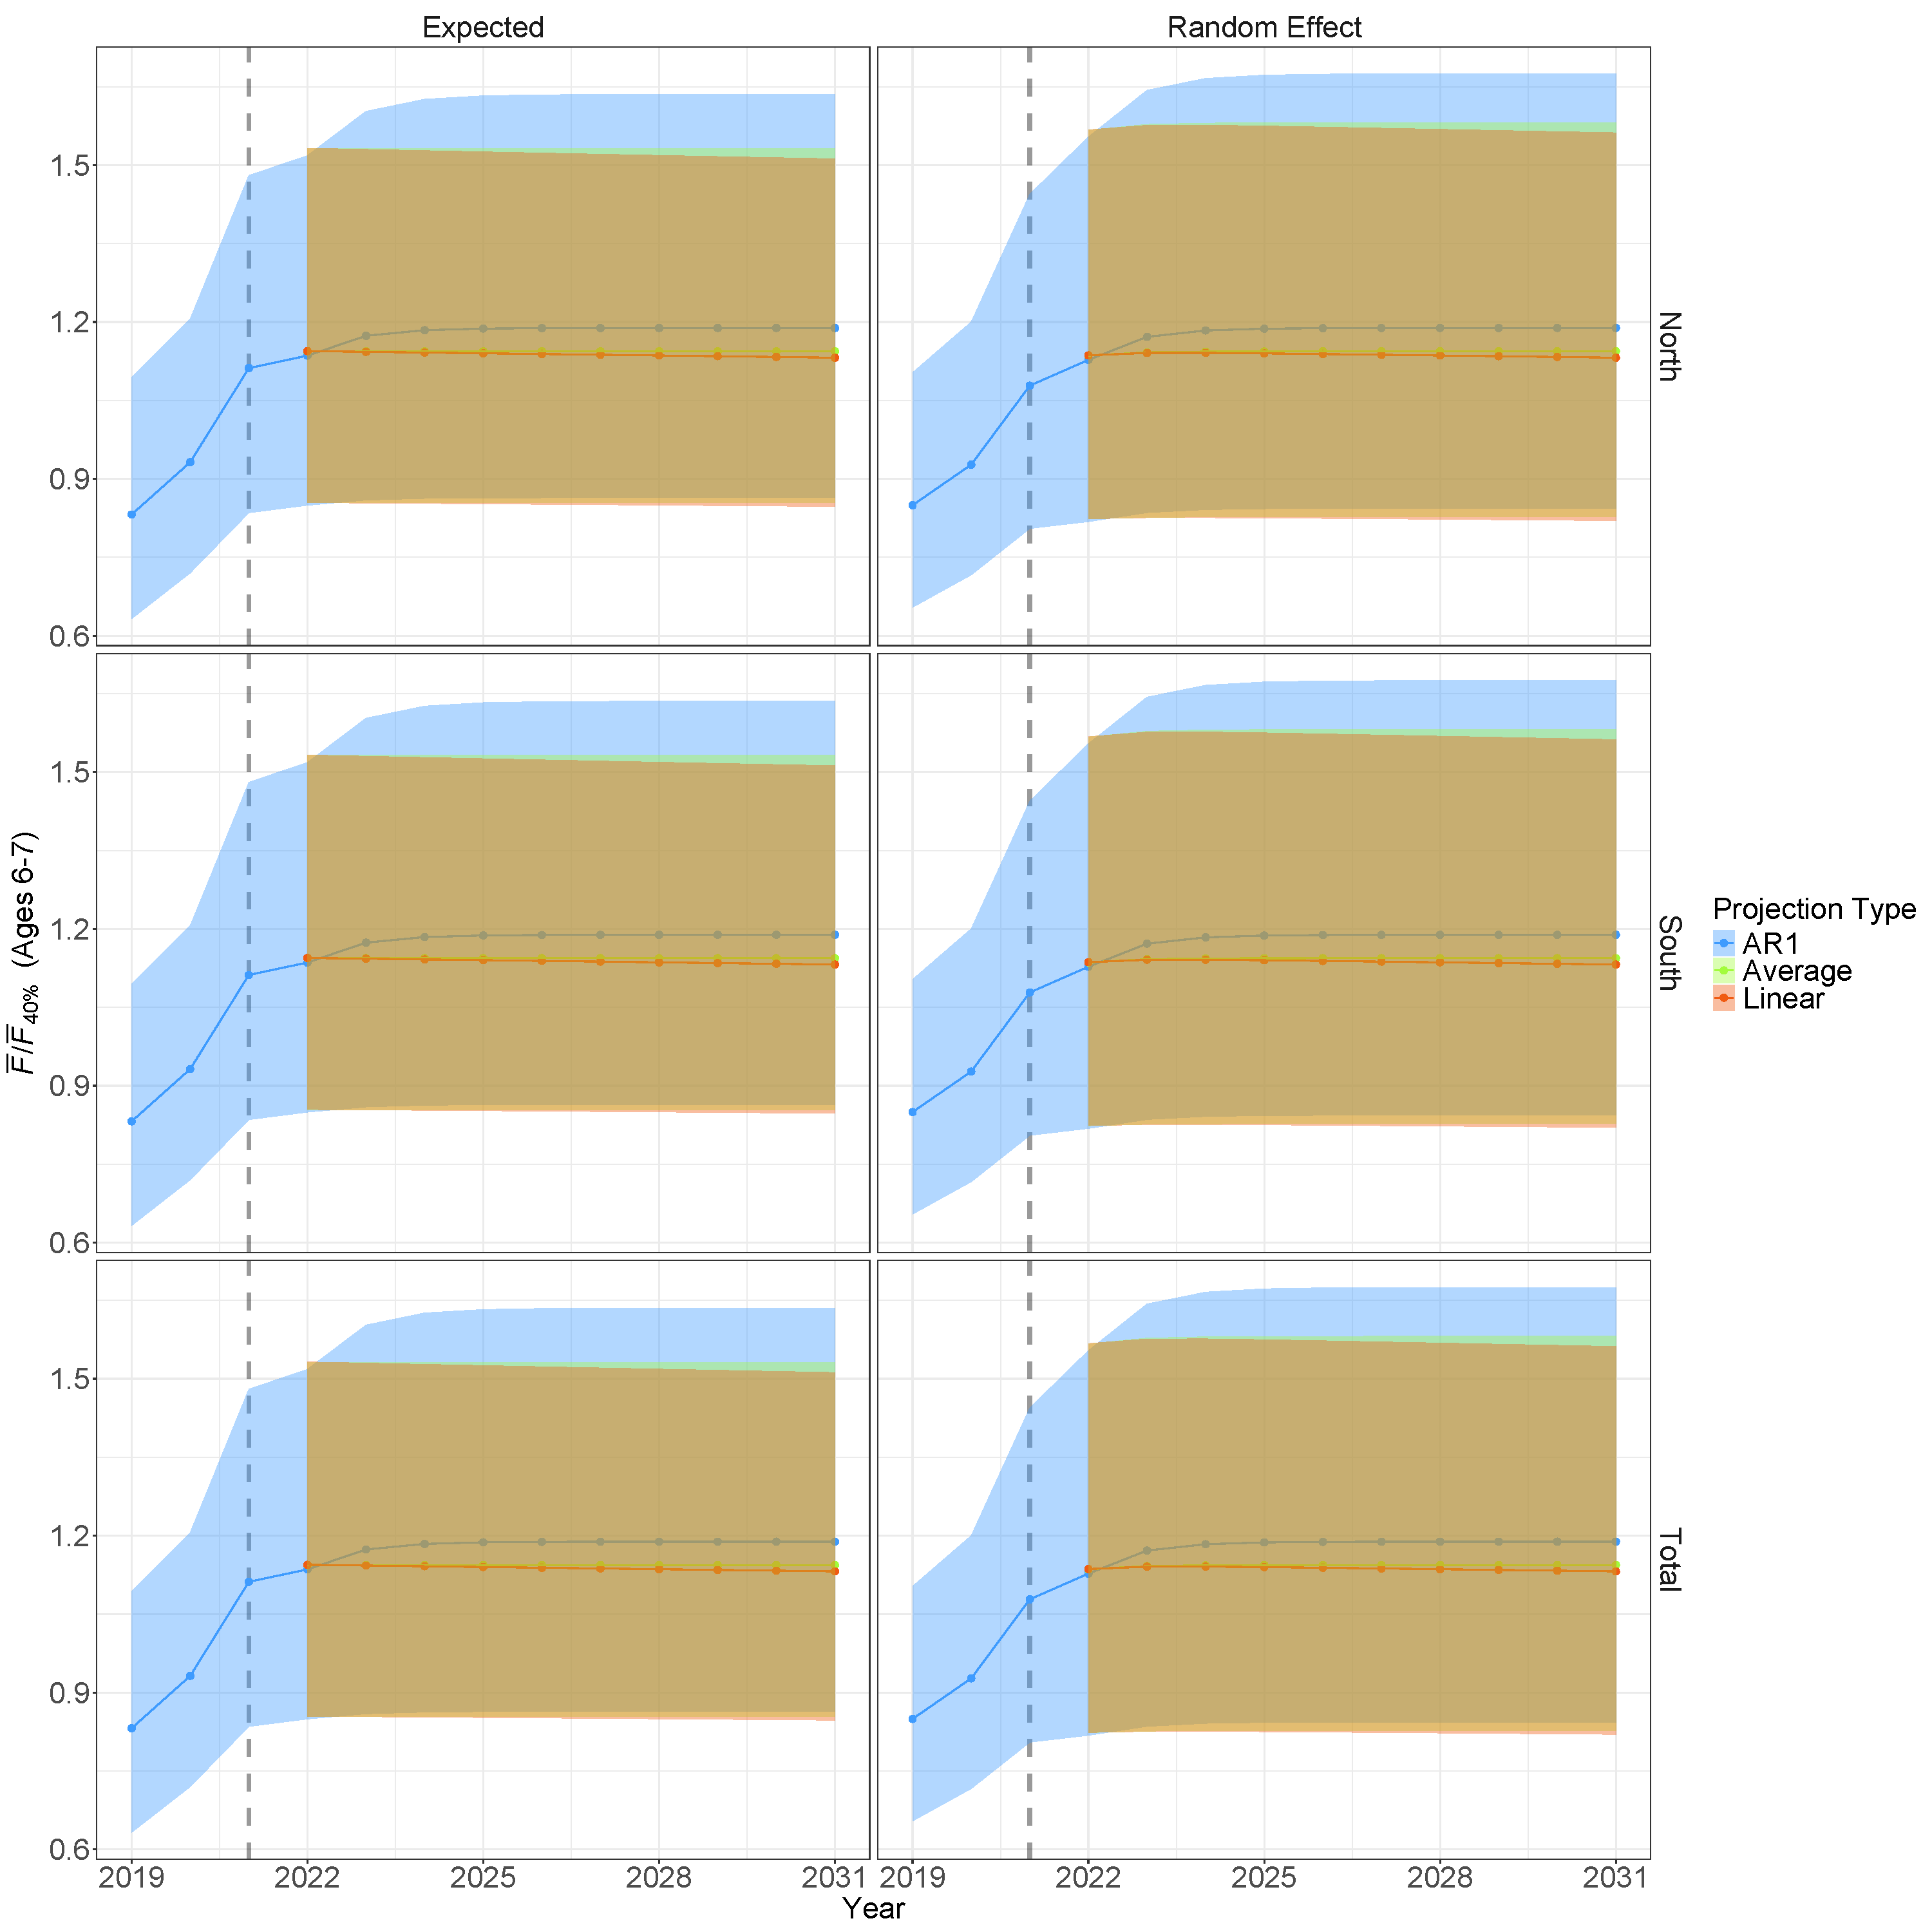
\includegraphics[height=0.95\textheight]{proj_F_status_results} 

}

\caption{Annual estimates of ratios of fishing mortality to $F_{40\%}$ by region and in total. Estimates in years beyond 2021 are from projecting model $M_1$ under alternative assumptions for bottom temperature anomalies in the northern region. Vertical dotted lines indicate the last year of data and polygons represent 95\% confidence intervals.}\label{fig:F-status-proj}
\end{figure}
\begin{figure}

{\centering 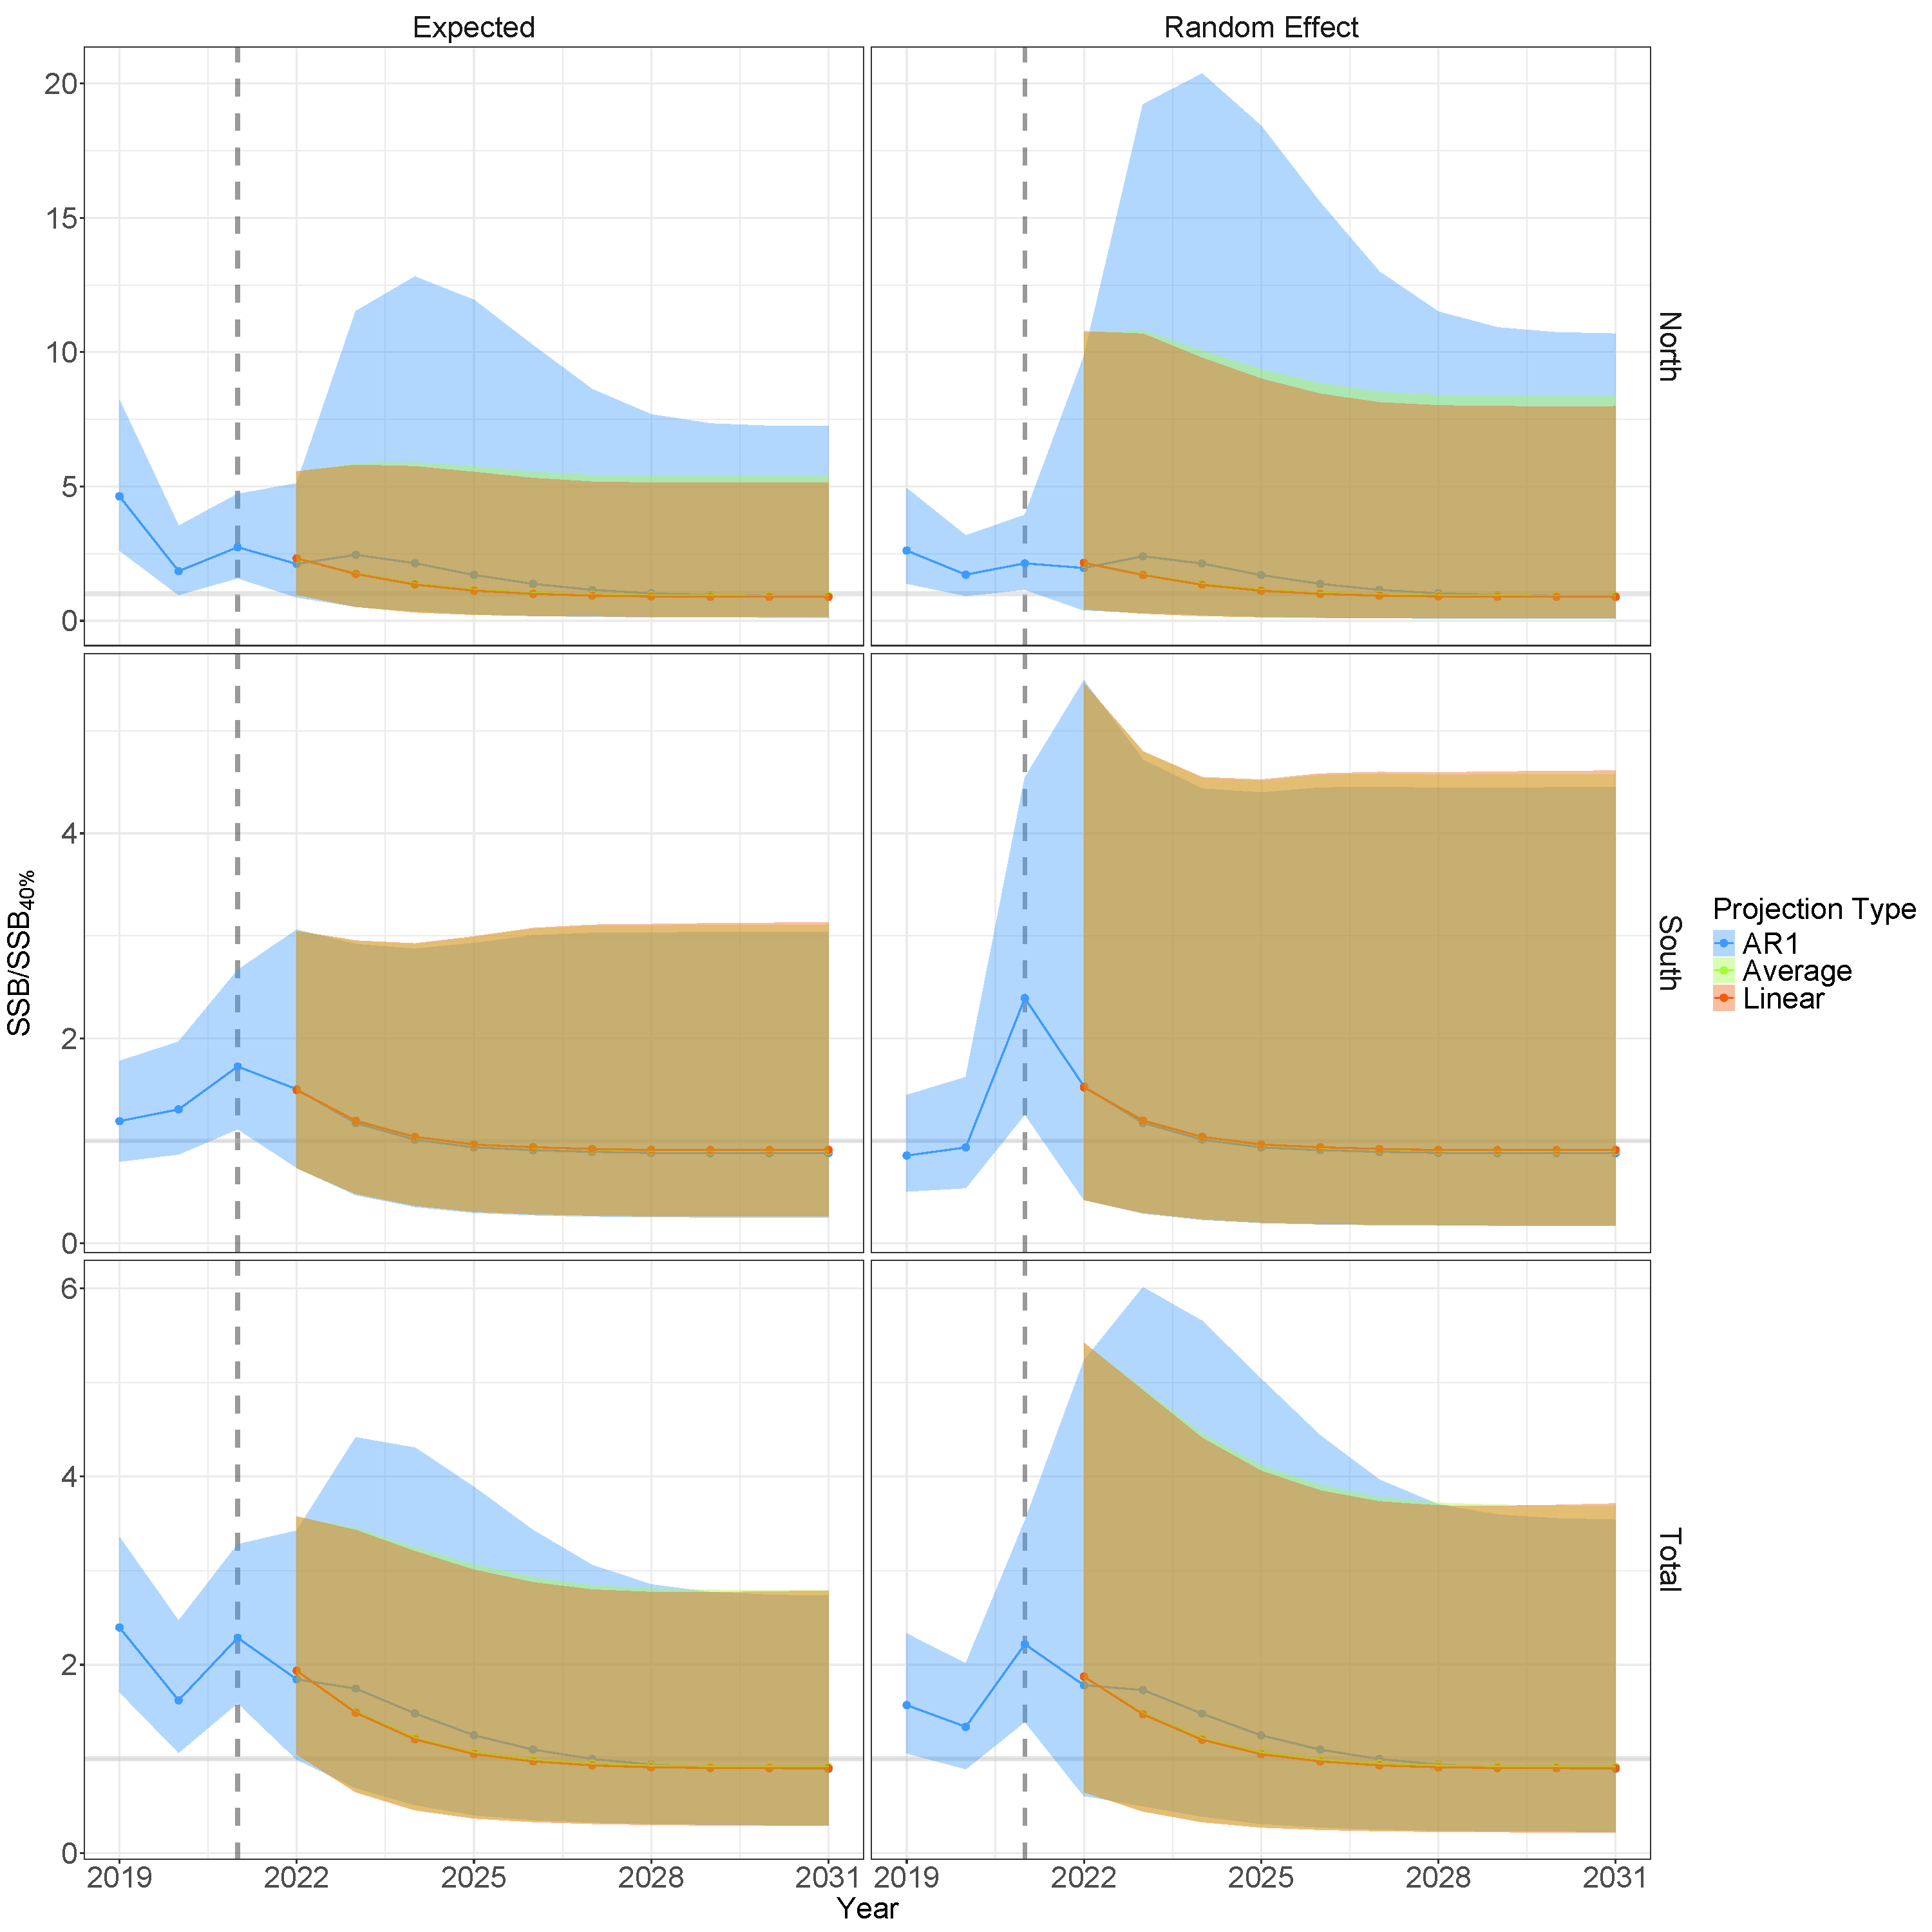
\includegraphics[height=0.95\textheight]{proj_SSB_status_results} 

}

\caption{Annual estimates of ratios of SSB to SSB$_{40\%}$ by region and in total. Estimates in years beyond 2021 are from projecting model $M_1$ under alternative assumptions for bottom temperature anomalies in the northern region. Vertical dotted lines indicate the last year of data and polygons represent 95\% confidence intervals.}\label{fig:SSB-status-proj}
\end{figure}

\end{document}
